%%%%%%%%%%%%%%%%%%%%%%%%%%%%%%%%%%%%
%Author: L.V. Fardigola (fardigola@karazin.ua), 
%Dept. of Applied Mathematics,
%V.N. Karazin Kharkiv National University, Kharkiv, Ukraine
%%%%%%%%%%%%%%%%%%%%%%%%%%%%%%%%%%%%%
\documentclass[14pt,a4paper,oneside]{extbook}
\usepackage{cmap}
\usepackage{amsthm,amsfonts,mathtools,amscd,amssymb, mathrsfs}
\usepackage{latexsym}
\usepackage{euscript}
\usepackage{multicol}
\usepackage{bbm}
%\usepackage{rotating}
\usepackage{graphicx}
%\usepackage{epstopdf}
\usepackage{tikz}
\usetikzlibrary{positioning, arrows.meta}
\usepackage{array}
\usepackage{caption}
\usepackage{subcaption}
\usepackage{cite}
\usepackage{listings}
\usepackage{setspace}
\usepackage{microtype}
%%%%%%%%%%%%%%%%%%%% languages %%%%%%%%%%%
\usepackage{fontspec}
\setmainfont{Times New Roman}
\setmonofont{DejaVu Sans Mono}
\renewcommand{\figurename}{Рисунок}
\renewcommand{\tablename}{Таблиця}
%%%%%%%%%%%%%%%%%%%%%%%%%%%%%%%%%%%%%%%%%%
\usepackage[
    unicode=true,     % Enable unicode support
    colorlinks=true,  % Enable link coloring
    linkcolor=black,  % Set internal links (like ToC entries) to black
    urlcolor=black,    % Optional: Keep URLs blue (or set to black)
    citecolor=black   % Changed from green to black
]{hyperref}           % Load hyperref (usually last or near last)
%%%%%%%%%%%%%%%
\usepackage[left=25mm, right=15mm, top=20mm, bottom=20mm]{geometry}
\tolerance=9000
%\textwidth=165mm
%\textheight=250mm
%\oddsidemargin=4.6mm
%\voffset=-20mm
\binoppenalty=1 \relpenalty=1
\allowdisplaybreaks
%\everymath{\displaystyle}
%\renewcommand{\baselinestretch}{1.44}
\onehalfspacing
\setcounter{secnumdepth}{3}
\setcounter{tocdepth}{3}
%%%%%%%%%%%%%%%%%%%%%%%%%%%
\usepackage{th-sty}
%%%%%%%%%%%%%%%%%%%%%%%%%
\usepackage{fancyhdr}
\pagestyle{fancy}
\fancyhf{}
\renewcommand{\headrulewidth}{0pt}
\renewcommand{\footrulewidth}{0pt}
\fancyhead[R]{\thepage}
\fancypagestyle{plain}{
  \fancyhf{}
  \renewcommand{\headrulewidth}{0pt}
  \renewcommand{\footrulewidth}{0pt}
  \fancyhead[R]{\thepage}
}
%%%%%%%%%%%%%%%%%%%%%%%%%
\graphicspath{ {pictures/} }
%%%%%%%%%%%%%%%%%%%%%%%%%%%%%%%%%%%%
\theoremstyle{dplplain}
\newtheorem{theorem}{Теорема}[chapter]
\newtheorem{corollary}[theorem]{Наслідок}%[chapter]
\newtheorem{statement}[theorem]{Твердження}%[chapter]
\newtheorem{lemma}[theorem]{Лема}%[chapter]
\theoremstyle{dpldefinition}
\newtheorem{definition}[theorem]{Означення}%[chapter]
\theoremstyle{dplremark}
\newtheorem{problem}[theorem]{Задача}%[chapter]
\newtheorem{remark}[theorem]{Зауваження}%[chapter]
\newtheorem{example}[theorem]{Приклад}%[chapter]
%%%%%%%%%%%%%%%%%%%%%%%%%%%%%%%%%%%%%%%
\newcommand{\R}{{\mathbb R}}
\newcommand{\RR}{\overline{\mathbb R}}
\newcommand{\N}{{\mathbb N}}
\newcommand{\Z}{{\mathbb Z}}
\renewcommand{\C}{{\mathbb C}}
\newcommand{\Q}{{\mathbb Q}}
%%%%%%%%%%%%%%%%%%%%%%%%%%%%%%%%%%%%%%%%%%%%%%%%%%%%%%%%%%
\newcommand{\fnnl}{\left[\!\left[\!\left|}
\newcommand{\fnnr}{\right|\!\right]\!\right]}
\newcommand{\fnl}{\left[\!\left|}
\newcommand{\fnr}{\right|\!\right]}
\newcommand{\nnnl}{\left|\!\left|\!\left|}
\newcommand{\nnnr}{\right|\!\right|\!\right|}
\newcommand{\nnl}{\left\|}
\newcommand{\nnr}{\right\|}
\newcommand{\nl}{\left|}
\newcommand{\nr}{\right|}
\newcommand{\pl}{\left(}
\newcommand{\pr}{\right)}
\newcommand{\bl}{\left[}
\newcommand{\br}{\right]}
\newcommand{\bbl}{\left\{}
\newcommand{\bbr}{\right\}}
\newcommand{\pnl}{\left(\kern-0.21em\left|}
\newcommand{\pnr}{\right|\kern-0.21em\right)}
\newcommand{\lal}{\left\langle}
\newcommand{\lar}{\right\rangle}
%%%%%%%%%%%%%%%%%%%%%%%%%%%%%%%%%%%%%%%%%%%%%%%%%%%%%%%%%%
\newcommand{\supp}{\mathop{\mathrm{supp}}}
\newcommand{\sign}{\mathop{\mathrm{sign}}}
\newcommand{\sinc}{\mathop{\mathrm{sinc}}}
\newcommand{\Ker}{\mathop{\mathrm{Ker}}}
\newcommand{\lin}{\mathop{\mathrm{lin}}}
\newcommand{\sgn}{\mathop{\mathrm{sgn}}}
\newcommand{\tr}{\mathop{\mathrm{tr}}}
\renewcommand{\Im}{\mathop{\mathrm{Im}}}
\renewcommand{\Re}{\mathop{\mathrm {Re}}}
\newcommand{\K}{\mathcal K}
\newcommand{\HH}{\mathcal H}
\newcommand{\m}{\mathsf{m}}
\newcommand{\mm}{\operatorname{\mathsf{mod}}}
\newcommand{\PP}{\mathcal P}
\newcommand{\PPP}{\overline{\mathcal P}}
\newcommand{\SSS}{\mathcal S}
\newcommand{\FF}{\mathcal F}
\newcommand{\LL}{\mathcal L}
\newcommand{\BB}{\mathcal B}
\newcommand{\one}{\mathbbmss 1}
\newcommand{\ubar}[1]{\text{\b{$#1$}}{}}
\newcommand{\V}{\mathbb V}
\newcommand{\BV}{\mathbb{BV}}
\newcommand{\AC}{\mathbb{AC}}
\newcommand{\midd}{\,\middle|\,}
%%%%%%%%%%%%%%%%%%%%%%%%
\DeclareMathOperator*{\esssup}{ess\,sup}
\DeclareMathOperator*{\essinf}{ess\,inf}
\DeclareMathOperator*{\bigtimes}{\mbox{\raisebox{-0.5ex}{\huge$\times$}}}
\DeclareMathOperator*{\smalltimes}{\mbox{\raisebox{-0.3ex}{\large$\times$}}}
\DeclareMathOperator*{\ootimes}{\overline{\otimes}}
%%%%%%%%%%%% LISTING %%%%%%%%%%%%%%%%%%%
\lstset{language=Python}
\lstset{frame=lines}
\lstset{basicstyle=\normalsize}
\lstset{prebreak=\raisebox{-2ex}[0ex][0ex]{\ensuremath{\hookleftarrow}}}
\lstset{breaklines=true}
\captionsetup[lstlisting]{font=large}

\renewcommand{\UrlFont}{\rmfamily\relax}

\begin{document}
\sloppy

\begin{titlepage}

    \begin{center}
        \textbf{КИЇВСЬКИЙ НАЦІОНАЛЬНИЙ УНІВЕРСИТЕТ \\[-0.3em]
        ІМЕНІ ТАРАСА ШЕВЧЕНКА} \\
        \normalsize
        {\medium Факультет комп’ютерних наук та кібернетики \\[-0.3em]
        Кафедра інтелектуальних програмних систем}
    \end{center}

    \vspace{0.01cm}

    \begin{center}
    \textbf{Кваліфікаційна робота \\[-0.3em]
    на здобуття ступеня магістра} \\[-0.3em]
    за спеціальністю \textbf{121 Інженерія програмного забезпечення} \\[-0.3em]
    на тему: \\
    \textbf{ЗАСТОСУВАННЯ ІДЕЇ ОДНОРАЗОВОГО БЛОКНОТУ \\
    У КІЛЬЦЯХ ЛИШКІВ}
    \end{center}

    \vspace{0.5cm}

    \noindent
    \mediuml
    \begin{tabular}{@{}p{0.9\textwidth}@{}p{0.58\textwidth}@{}}
        Виконав студент 2-го курсу & \\[-0.3em]
        ОНП «Програмне забезпечення систем» & \\[-0.3em]
        Рябов Кирило Сергійович & \hspace{-1.7cm}\rule{2.5cm}{0.5pt} \\[-0.6em]
        & \hspace{-1.25cm} {\medium (підпис) } \\[0.2em]

        Науковий керівник: & \\[-0.3em]
        професор кафедри інтелектуальних програмних систем & \\[-0.3em]
        доктор фізико-математичних наук, професор & \\[-0.3em]
        Кривий Сергій Лук'янович & \hspace{-1.7cm}\rule{2.5cm}{0.6pt} \\[-0.6em]
        & \hspace{-1.25cm} {\medium (підпис) } \\[1.5em]
    \end{tabular}

    \noindent
    \mediuml
    \begin{tabular}{@{}p{0.35\textwidth}@{}p{0.7\textwidth}@{}}
        & Засвідчую, що в цій роботі \\[-0.3em]
        & немає запозичень з праць інших авторів \\[-0.3em]
        & без відповідних посилань. \\[-0.3em]
        & Студент \hspace{5.8cm}\rule{2.5cm}{0.6pt}\\[-0.6em]
        & \hspace{8.1cm} {\medium (підпис) } \\[1.5em]

        & Роботу розглянуто й допущено до захисту на \\[-0.3em]
        & засіданні кафедри інтелектуальних програмних \\
        & систем \\
        & «\rule{1.5cm}{0.4pt}» \rule{3cm}{0.4pt} 2025 р., \\
        & протокол № \rule{2cm}{0.4pt} \\
        & Завідувач кафедри \\
        & доктор фіз.-мат. наук, професор \\
        & Олександр ПРОВОТАР \hspace{2.55cm}\rule{2.5cm}{0.6pt}\\[-0.6em]
        & \hspace{8.1cm} {\medium (підпис) } \\
    \end{tabular}

    \vfill

    \begin{center}
        КИЇВ 2025
    \end{center}
\end{titlepage}


\refstepcounter{page}

\begin{center}
    \textbf{РЕФЕРАТ}
\end{center}

Обсяг роботи 62 сторінки, 8 ілюстрацій, 5 таблиць, 23 джерела.

СКІНЧЕННІ КІЛЬЦЯ, СИМЕТРИЧНА КРИПТОСИСТЕМА, СЮР’ЄКТИВНІ ВІДОБРАЖЕННЯ, СИСТЕМИ ЛІНІЙНИХ РІВНЯНЬ, ІЗОМОРФІЗМ КІЛЕЦЬ,
КОМБІНАТОРНА КРИПТОСТІЙКІСТЬ, ПРОГРАМНА РЕАЛІЗАЦІЯ, ВЕРИФІКОВАНІ ОБЧИСЛЕННЯ.

Об’єктом дослідження є процес симетричного шифрування інформації на основі алгебраїчних структур скінченних кілець та систем лінійних рівнянь.

Предметом роботи є розробка симетричної криптосистеми, що використовує сюр’єктивні відображення між кільцями та афінні
перетворення для забезпечення захисту даних.

Метою роботи є створення, теоретичне обґрунтування та програмна реалізація симетричної криптосистеми, що використовує
сюр'єктивні відображення скінченних кілець та їх ізоморфізми з використанням систем лінійних рівнянь над кільцями лишків.

У роботі застосовано методи теоретичного аналізу алгебраїчних структур, комбінаторики відображень, побудови та дослідження алгоритмів.
Програмна реалізація виконана мовою Rust із використанням інтегрованого середовища RustRover IDE для реалізації бібліотеки.

У результаті розроблено алгоритм GEN-G для генерації скінченних кілець та ізоморфізмів, описано та реалізовано протокол
симетричного шифрування/дешифрування з багаторівневою обфускацією даних, проведено теоретичний аналіз стійкості, створено
програмну бібліотеку для генерації кілець, шифрування та дешифрування.
Досліджено можливості застосування системи у верифікованих обчисленнях із доказами з нульовим розголошенням.

Розроблений програмний продукт може бути впроваджений для симетричного шифрування даних у випадках, коли сторони можуть
безпечно узгодити спільний ключ, а також у пристроях з обмеженими ресурсами (IoT, смарт-картки).

Результати роботи можуть бути використані для подальшого розвитку симетричних криптосистем на основі алгебраїчних структур,
а також для інтеграції з сучасними протоколами захисту інформації.
Доцільним є продовження досліджень щодо оптимізації продуктивності, розширення сфери застосування та впровадження в існуючі системи.

\renewcommand{\contentsname}{ЗМІСТ}
\renewcommand{\cfttoctitlefont}{\centering\bfseries\MakeUppercase}
\renewcommand{\aftertoctitle}{\\[1.5em]}

\tableofcontents

\begin{center}
{\Large \textbf{СКОРОЧЕННЯ ТА УМОВНІ ПОЗНАКИ}}
\end{center}

\vspace{1.5\baselineskip}

{\Large

\noindent БЗ --- база знань; \\
БНФ --- Бекуса-Наура форма; \\
ВІС --- виконавча інформаційна система; \\
ВП --- віртуальне підприємство;

}


\chapter*{ВСТУП}
\phantomsection
\addcontentsline{toc}{chapter}{ВСТУП}

{\Large

Оцінка сучасного стану об’єкта розроблення. Правильно організована
навчально-пізнавальна діяльність --- це головне джерело розвитку пізнавальних
інтересів, активності, самоорганізації та творчого мислення, забезпечення єдності
інтелектуального й особистісного розвитку. Інформатизація освіти й зростаючі
вимоги до якості та кількості висококваліфікованих фахівців створюють
необхідність розробки та впровадження інноваційних освітніх методик і
технологій.

Підвищення теоретичного рівня курсу фізики, інтеграція знань, новітні
засоби і форми навчання спонукають до подальших пошуків можливостей
застосування ЕОМ у навчальному процесі як стимулюючого та інтенсифікуючого
чинника.

Інформаційні технології навчання передбачають широке використання
комп'ютерної техніки та спеціального програмного забезпечення як потужного
засобу навчання фізики. Проблемами впровадження інформаційних технологій у
навчальний процес з фізики займалися: О. Бугайов, Є. Коршак, М. Головко, В.
Заболотний, Ю. Жук, О. Ляшенко, Н. Сосницька, М. Шут та ін. У працях [1--5] цих % Use -- for en-dash in ranges
вчених розглядаються питання удосконалення шкільного фізичного експерименту
засобами інформаційних технологій; поєднання традиційних засобів навчання,
зокрема підручника з фізики, з електронними; розробки ППЗ з вивчення окремих
тем курсу фізики. При роботі з ЕОМ створюється специфічний емоційний
настрій, формується алгоритмічна культура [2; 6].

Актуальність роботи та підстави для її виконання. При вивченні фізики
нерідко складається ситуація, коли учень на практиці не може застосувати набуті
знання, навіть у випадку їх осмисленого засвоєння. Отже, необхідно навчати
практичному використанню набутих знань й умінь [3; 4].

Реалізувати інтеграцію теоретичних знань та практичних навичок доцільно
шляхом залучення учнів до розв’язування дослідницько-творчих задач. Тому
актуальним є створення засобів, які за допомогою експериментальних задач
забезпечують оволодіння повноцінними вміннями. Завдання на розрахунок опору
електричного кола можна зустріти серед екзаменаційних та олімпіадних задач, а
також у завданнях зовнішнього незалежного оцінювання.

\textbf{Мета й завдання роботи.} Метою кваліфікаційної роботи є створення
програмного засобу для розв’язування задач на розрахунок опору електричного
кола. Для досягнення цієї мети поставлено такі завдання.
% Use the itemize environment for bulleted lists
\begin{itemize}
    \item Дослідити існуючі електронні засоби навчання фізики.
    \item Дослідити застосування різних способів розрахунку опору
    електричного кола.
    \item Розробити технічне завдання до продукту.
    \item Розробити інтерфейс та дизайн програмного продукту «Навчальна
    система для відображення та обчислення опору ділянки електричного
    кола».
\end{itemize}

Об'єкт, методи й засоби розроблення. Об’єктом розроблення програмного
засобу «Навчальна система для відображення та обчислення опору ділянки
електричного кола» є процес розв’язування задач на визначення опору
електричного кола за допомогою програмного засобу.

Розробленню програмного засобу передувало створення математичної
моделі задач на визначення опору електричного кола. Основу для цього склав
аналіз деяких типів з’єднання елементів та систематизація відповідних методів
обчислення опору.

Під час розроблення програмного продукту використана еволюційна
модель, заснована на таких принципах. Розробляється початкова версія продукту,
яка передається кінцевим користувачам для оцінки, після чого продукт
доробляється, враховуючи думку замовника. Аналогічно розробляються,
передаються й оцінюються проміжні версії програмного продукту, поки не
з’явиться повністю готовий продукт, який відповідає всім вимогам замовника.
Процеси специфікації, розробки та атестації програмного продукту ведуться
паралельно з постійним обміном інформації між ними.

В якості інструменту створення програмного засобу було обрано NetBeans
IDE 7.2.1 --- інтегроване середовище розробки (IDE) мовою програмування Java,
яке є безкоштовним, вільно поширюваним, з відкритим вихідним кодом.

Можливі сфери застосування. Програмний продукт «Навчальна система
для відображення та обчислення опору ділянки електричного кола» може
застосовуватися в навчальному процесі в шкільному курсі фізики під час
вивчення опору в електричному колі.

Взаємозв’язок з іншими роботами. Ця робота є частиною великого
спільного проєкту, що охоплював розроблення навальних засобів для різних
задач шкільної фізики, алгебри та хімії.

}


\chapter{ТЕОРЕТИЧНЕ ПІДҐРУНТЯ КРИПТОСИСТЕМИ}\label{ch:-1:---}

У цьому розділі викладено основні теоретичні положення, що лежать в основі розробки та аналізу симетричної криптосистеми, запропонованої у цій роботі.


\section{Вступ до основ криптографії}
\label{sec:crypto_intro}

Криптографія пройшла шлях від простих шифрів заміни, що використовувалися ще в античності (наприклад, шифр Цезаря),
до сучасних протоколів захисту інформації (зокрема, TLS, системи наскрізного шифрування).
Основними завданнями криптографії є забезпечення конфіденційності (захист від несанкціонованого доступу),
цілісності (контроль змін) та автентифікації (верифікація ідентичності).

Побудова надійних криптосистем ґрунтується на двох фундаментальних принципах:
\begin{itemize}
    \item \emph{Принцип Керкгоффса}~\cite{Kerckhoffs83}: Безпека криптосистеми не повинна залежати від секретності алгоритму;
    достатньо зберігати в таємниці лише ключ.
    \item \emph{Досконала секретність за Шенноном}~\cite{Shannon49}: Шифр вважається досконалим, якщо шифротекст не містить жодної
    інформації про відкритий текст (наприклад, одноразовий блокнот за умови випадковості ключа).
\end{itemize}

К. Шеннон також увів поняття \emph{перемішування} (confusion) та \emph{розсіювання} (diffusion), які реалізуються у сучасних
блокових шифрах (наприклад, AES) через мережі підстановок і перестановок~\cite{Shannon49}.

Ці високорівневі концепції лежать в основі розробленої криптосистеми.

\subsection{Базові поняття та означення}
\label{subsec:crypto_basics}

Для повного розуміння розробленої системо розглянемо наступні означення~\cite{Mao04,BerczesEtAl14}:

\begin{description}
    \item[Криптосистема:] Трійка алгоритмів \((\mathsf{KeyGen},\mathsf{Encrypt},\mathsf{Decrypt})\), що працюють за поліноміальний час відносно параметра безпеки \(n\).
    \(\mathsf{KeyGen}\) генерує ключі; \(\mathsf{Encrypt}(K,P)\) перетворює відкритий текст \(P\) у шифротекст \(C\); \(\mathsf{Decrypt}(K,C)\) відновлює \(P\).
    \item[Відкритий текст (\(P\)):] Початкове повідомлення.
    \item[Шифротекст (\(C\)):] Закодований результат, що приховує \(P\).
    \item[Ключ (\(K\)):] Секретний параметр, що визначає відображення шифрування та розшифрування.
    \item[Шифрування:] Операція \(C \leftarrow \mathsf{Encrypt}(K,P)\).
    \item[Розшифрування:] Операція \(P \leftarrow \mathsf{Decrypt}(K,C)\), причому \\ \(\mathsf{Decrypt}(K, \mathsf{Encrypt}(K,P)) = P\).
    \item[Криптоаналіз:] Методи відновлення \(K\) або \(P\) з \(C\) без авторизованого доступу.
\end{description}

Для кращого розуміння вище наведених визначень розглянемо наступний приклад.

\begin{example}[Шифр Вернама / Одноразовий блокнот]
    \label{ex:otp_vernam}
    Цей симетричний шифр, також відомий як одноразовий блокнот (One-Time Pad, OTP), був запропонований Гільбертом Вернамом.
    Нехай відкритий текст \(P\), шифротекст \(C\) та ключ \(K\) є бінарними послідовностями однакової довжини \(n\), тобто \(P, C, K \in \{0, 1\}^n\).
    Операції шифрування та розшифрування виконуються побітово за допомогою операції XOR (\(\oplus\), що еквівалентно додаванню за модулем 2):
    \begin{itemize}
        \item Шифрування: \(C = P \oplus K\) (тобто \(C_i = P_i \oplus K_i\) для \(i=1, \dots, n\)).
        \item Розшифрування: \(P = C \oplus K\) (оскільки \(C \oplus K = (P \oplus K) \oplus K = P \oplus (K \oplus K) = P \oplus 0 = P\)).
    \end{itemize}
    Шифр Вернама забезпечує досконалу секретність за Шенноном, тобто є теоретично невразливим, за умови суворого дотримання таких вимог до ключа \(K\):
    \begin{enumerate}
        \item Ключ \(K\) має бути абсолютно випадковою послідовністю.
        \item Довжина ключа \(|K|\) повинна бути не меншою за довжину відкритого тексту \(|P|\).
        \item Ключ \(K\) повинен використовуватися для шифрування лише одного повідомлення (одноразове використання).
    \end{enumerate}
    Порушення будь-якої з цих умов робить шифр вразливим.
    Основною практичною складністю є генерація та безпечна передача довгих, випадкових одноразових ключів~\cite{Shannon49}.
\end{example}

Криптографічні системи можемо поділити на \emph{симетричні криптосистеми}, де один і той самий секретний ключ \(K\) використовується для шифрування і розшифрування.
До прикладів можемо віднести: шифр Вернама (який наведено як приклад вище), AES, ChaCha20.
Та на \emph{Асиметричні криптосистеми} (з відкритим ключем), де для шифрування використовується відкритий ключ \(K_{\text{pub}}\), а для розшифрування — приватний ключ \(K_{\text{priv}}\).
До прикладів можемо віднести RSA, ElGamal encryption.

Запропонована система належить до симетричних і ґрунтується на сюр'єктивних відображеннях скінченних кілець та їх ізоморфізмів з використанням систем лінійних рівнянь над кільцями лишків.

\subsection{Мотивація та підхід створення криптосистеми}
\label{subsec:motivation}

Метою цієї роботи є розробка криптосистеми, що базується на об'єктах порівняно невеликих розмірів і забезпечує достатній рівень стійкості до злому.
Можна виділити наступні ключові характеристики системи:

\begin{enumerate}
    \item \emph{Обчислювальна ефективність:} Використання малого модуля \(k\) зменшує вартість арифметичних операцій.
    \item \emph{Простота реалізації:} Скінченні кільця \(\mathbb{Z}_k\) легко реалізуються на пристроях з обмеженими ресурсами (наприклад, смарт-карти, IoT).
    \item \emph{Комбінаторна стійкість:} Кількість сюр'єктивних гомоморфізмів \(\mathbb{Z}_k \to \mathbb{Z}_\ell\) та ізоморфізмів кілець швидко зростає зі зростанням кількості дільників \(k\), що ускладнює криптоаналіз.
    \item \emph{Стійкість до статистичних атак:} Вбудовування відкритого тексту у системи лінійних рівнянь над \(\mathbb{Z}_k\) ускладнює застосування частотного аналізу та подібних методів.
\end{enumerate}

Запропонована схема розвиває ідеї симетричного протоколу обміну~\cite{KryvyiEtAl22}, доповнюючи їх кільцевими перетвореннями та афінними відображеннями систем лінійних рівнянь.


\section{Основи теорії кілець}
\label{sec:ring_theory}

Кільця становлять алгебраїчну основу для побудови криптосистеми.
У цьому підрозділі наведено їхні означення, властивості та приклади, що мають значення для подальшого викладу.

\subsection{Означення та властивості кілець}
\label{subsec:ring_definition}

\begin{definition}
    \label{def:ring}
    \emph{Кільце} \((R,+,\cdot)\) — це множина \(R\) з двома бінарними операціями, для яких виконуються такі умови:
    \begin{enumerate}
        \item \((R,+)\) — абелева група з нульовим елементом \(0\) та протилежним елементом \(-a\) для кожного \(a\in R\).
        \item \((R,\cdot)\) — моноїд з одиницею \(1\): множення асоціативне (\(a(bc)=(ab)c\)), існує \(1\in R\) таке, що \(1\cdot a = a\cdot 1 = a\) для всіх \(a\in R\).
        \item \emph{Розподільність:} для всіх \(a,b,c\in R\)
        \[
            a\cdot(b + c) = ab + ac, \quad (b + c)\cdot a = ba + ca.
        \]
    \end{enumerate}
    Якщо множення комутативне (\(ab=ba\)), кільце називають \emph{комутативним}.
    Якщо \(R\) скінченне, комутативне та має одиницю \(1\neq0\), таке кільце називають \emph{скінченним комутативним кільцем з одиницею}.
\end{definition}

Основні поняття, пов'язані з кільцями:
\begin{description}
    \item[Дільник нуля:] Елемент \(a\neq0\), для якого існує \(b\neq0\) такий, що \(ab=0\).
    \item[Дільник одиниці (оборотний елемент):] Елемент \(u\in R\), для якого існує обернений \(u^{-1}\) такий, що \(uu^{-1}=u^{-1}u=1\).
    Множина всіх дільників одиниці утворює групу відносно множення, позначається \(R^\times\).
    \item[Характеристика:] Найменше натуральне \(n>0\), для якого \(n\cdot1 = 0\) (тобто \(1+\dots+1=0\), \(n\) разів).
    Якщо такого \(n\) не існує, характеристика дорівнює нулю.
\end{description}

\subsection{Кільця лишків за модулем \(k\) (\(\mathbb{Z}_k\))}
\label{subsec:residue_rings}

Нехай \(k\ge2\) — ціле число.
Кільце лишків за модулем \(k\) — це множина класів конгруентності за модулем \(k\):
\[
    \mathbb{Z}_k = \{\bar{0},\bar{1},\dots,\overline{k-1}\}, \quad \text{де } \bar{a} = a + k\mathbb{Z} = \{x\in\mathbb{Z} : x \equiv a \pmod{k}\}.
\]
Операції визначаються так:
\[
    \bar{a} + \bar{b} = \overline{a + b}, \quad \bar{a}\cdot\bar{b} = \overline{a\cdot b},
\]
тобто додавання та множення виконуються за модулем \(k\).
\((\mathbb{Z}_k, +, \cdot)\) — скінченне комутативне кільце з одиницею \(\bar{1}\).

\begin{example}[Операції в \(\mathbb{Z}_8\)]
    \label{ex:z8_ops}
    У кільці \(\mathbb{Z}_8\):
    \begin{gather*}
        \bar{3} + \bar{6} = \overline{3 + 6} = \overline{9} \equiv \bar{1} \pmod{8}.\\
        \bar{3}\cdot\bar{6} = \overline{3 \cdot 6} = \overline{18} \equiv \bar{2} \pmod{8}.\\
    \end{gather*}
    Дільники одиниці: \(\mathbb{Z}_8^\times = \{\bar{a} \in \mathbb{Z}_8 : \gcd(a,8)=1\} = \{\bar{1},\bar{3},\bar{5},\bar{7}\}\).
    Дільники нуля: \(\{\bar{a} \in \mathbb{Z}_8 \setminus \{\bar{0}\} : \gcd(a,8)>1\} = \{\bar{2},\bar{4},\bar{6}\}\).
    Наприклад, \(\bar{2}\cdot\bar{4} = \bar{8} \equiv \bar{0} \pmod{8}\).
\end{example}

\begin{example}[Ізоморфізм кілець]
    \label{ex:crt_iso}
    За китайською теоремою про лишки, якщо \(k={k_1k_2}\) і \(\gcd(k_1,k_2)=1\), то кільця \(\mathbb{Z}_k\) та \(\mathbb{Z}_{k_1} \times \mathbb{Z}_{k_2}\) є ізоморфними: \(\mathbb{Z}_k \cong \mathbb{Z}_{k_1} \times \mathbb{Z}_{k_2}\).
    Наприклад, \(\mathbb{Z}_6 \cong \mathbb{Z}_2 \times \mathbb{Z}_3\).
    Ізоморфізм \(\psi: \mathbb{Z}_6 \to \mathbb{Z}_2 \times \mathbb{Z}_3\) задається як \(\psi(\bar{a}) = (\overline{a \bmod 2}, \overline{a \bmod 3})\).
    Наприклад, \(\psi(\bar{5}) = (\overline{5 \bmod 2}, \overline{5 \bmod 3}) = (\bar{1}, \bar{2})\).
\end{example}

Позначимо через \(G_k\) будь-яке кільце, ізоморфне \(\mathbb{Z}_k\), з фіксованим ізоморфізмом \(\varphi: G_k \to \mathbb{Z}_k\).

\subsection{Мультиплікативна група дільників одиниці}
\label{subsec:ring_units_group}

Множина дільників одиниці \(\mathbb{Z}_k^\times\) утворює групу відносно множення за модулем \(k\):
\[
    \mathbb{Z}_k^\times = \{\bar{a}\in\mathbb{Z}_k : \gcd(a,k)=1\}.
\]
Ця група є абелевою.
Її порядок дорівнює \(\varphi(k)\), де \(\varphi\) — функція Ойлера.

\begin{example}[Група \(\mathbb{Z}_{10}^\times\)]
    \label{ex:z10_units}
    У \(\mathbb{Z}_{10}\), дільники одиниці: \(\mathbb{Z}_{10}^\times = \{\bar{1},\bar{3},\bar{7},\bar{9}\}\).
    Порядок групи \(\varphi(10) = 4\).
    Операція — множення за модулем 10.
    Наприклад, \(\bar{3}\cdot\bar{7} = \overline{21} \equiv \bar{1} \pmod{10}\), отже \(\bar{7} = \bar{3}^{-1}\).
    Група \(\mathbb{Z}_{10}^\times\) є циклічною, оскільки \(\bar{3}\) є генератором групи.
\end{example}

\begin{theorem}[Гаус~\cite{Shoup08}]
    \label{thm:cyclic_units}
    Група \(\mathbb{Z}_k^\times\) є циклічною тоді і тільки тоді, коли \(k=1,2,4,p^m\) або \(k=2p^m\), де \(p\) — непарне просте число, \(m\geq1\).
\end{theorem}

\subsection{Відображення між кільцями}
\label{subsec:ring_mappings}

Розглядаються такі типи відображень між кільцями:

\begin{description}
    \item[Гомоморфізм \(\phi: R\to S\):] Відображення, що зберігає операції: \(\phi(a+b)=\phi(a)+\phi(b)\) та \(\phi(a\cdot b)=\phi(a)\cdot\phi(b)\) для всіх \(a,b\in R\).
    \item[Ізоморфізм \(\varphi: R\to S\):] Бієктивний гомоморфізм.
    Якщо існує ізоморфізм, кільця \(R\) і \(S\) структурно еквівалентні (\(R\cong S\)).
    \item[Сюр'єкція (епіморфізм) \(\psi: R\to T\):] Гомоморфізм, образ якого збігається з усім \(T\) (\(\mathrm{Im}\,\psi = T\)).
    \item[Бієкція \(\psi_1: R\to R'\):] Взаємно однозначне відображення між множинами \(R\) та \(R'\), яке не обов'язково зберігає операції кілець.
\end{description}

\subsection{Ідеали та фактор-кільця}
\label{subsec:factor_rings}

Нехай \(R\) — кільце. Для побудови фактор-кільця необхідно ввести поняття ідеалу.

\textbf{Ідеал.} Підмножина \(I \subseteq R\) називається \emph{ідеалом} кільця \(R\), якщо виконуються такі умови:
\begin{itemize}
    \item \(I\) є підгрупою відносно додавання: для будь-яких \(a, b \in I\) маємо \(a-b \in I\);
    \item \(I\) замкнена відносно множення на довільний елемент кільця: для будь-яких \(r \in R\), \(a \in I\) маємо \(ra \in I\) і \(ar \in I\).
\end{itemize}
Ідеал можна розглядати як "узагальнення" поняття кратних у кільці цілих чисел: наприклад, множина всіх чисел, кратних \(n\), є ідеалом у \(\mathbb{Z}\).

\textbf{Фактор-кільце.} Нехай \(I\) — ідеал у кільці \(R\). \emph{Фактор-кільце} \(R/I\) — це множина всіх класів суміжності за ідеалом \(I\), тобто множина підмножин вигляду:
\[
    a + I = \{a + r : r \in I\}, \quad \text{де } a \in R.
\]
Кожен елемент \(R\) належить рівно одному такому класу.

Операції додавання та множення на \(R/I\) визначаються так:
\begin{gather*}
    (a + I) + (b + I) = (a + b) + I, \\
    (a + I) \cdot (b + I) = (ab) + I.
\end{gather*}
Ці операції коректно визначені, тобто не залежать від вибору представників класів.

\textbf{Властивість.} Фактор-кільце \(R/I\) саме є кільцем, а природне відображення \(\pi: R \to R/I\), \(\pi(a) = a + I\), є гомоморфізмом кілець з ядром \(I\).

\textbf{Теорема про ізоморфізм.} Якщо \(\psi: R \to T\) — сюр'єктивний гомоморфізм кілець, то фактор-кільце \(R/\ker\psi\) ізоморфне образу \(\psi\), тобто \(R/\ker\psi \cong \mathrm{Im}(\psi)\). Зокрема, якщо \(\psi\) сюр'єктивне, то \(R/\ker\psi \cong T\).

Таким чином, фактор-кільце дозволяє \texttt{"}розділити\texttt{"} кільце на класи за ідеалом і отримати нову алгебраїчну структуру, яка часто має простішу або більш зручну для застосування будову.

\section{Системи лінійних рівнянь над кільцями}
\label{sec:sle_theory}

У цьому підрозділі розглядаються системи лінійних рівнянь (СЛР) над скінченними комутативними кільцями.

\subsection{Означення та матричний запис}
\label{subsec:sle_definition}

Нехай \(R = \mathbb{Z}_m\) — скінченне комутативне кільце з одиницею.
\emph{Система з \(n\) лінійних рівнянь з \(n\) невідомими} над \(R\) має вигляд:
\[
    \begin{cases}
        a_{11}x_1 + a_{12}x_2 + \cdots + a_{1n}x_n \;\equiv\; b_1 \pmod{m},\\
        a_{21}x_1 + a_{22}x_2 + \cdots + a_{2n}x_n \;\equiv\; b_2 \pmod{m},\\
        \quad\vdots\\
        a_{n1}x_1 + a_{n2}x_2 + \cdots + a_{nn}x_n \;\equiv\; b_n \pmod{m},
    \end{cases}
\]
де коефіцієнти \(a_{ij} \in \mathbb{Z}_m\), вільні члени \(b_i \in \mathbb{Z}_m\), а невідомі \(x_j\) шукаються в \(\mathbb{Z}_m\).

У матричному записі ця система має вигляд:
\[
    A\,x \;\equiv\; b \pmod{m},
\]
де \(A = (a_{ij})\) — матриця розміру \(n\times n\) з елементами з \(\mathbb{Z}_m\), \(x = (x_j)\) — стовпчиковий вектор невідомих розміру \(n\times 1\), \(b = (b_i)\) — стовпчиковий вектор вільних членів розміру \(n\times 1\).

\subsection{Лінійні діофантові рівняння та конгруенції}
\label{subsec:diophantine}

\emph{Лінійне діофантове рівняння} — це рівняння вигляду \(a_1 x_1 + \dots + a_k x_k = c\) з цілими коефіцієнтами \(a_i, c \in \mathbb{Z}\), де шукаються цілі розв'язки \((x_1,\dots,x_k)\)~\cite{KameswariEtAl21}.
Система лінійних конгруенцій за модулем \(m\), як визначено вище, тісно пов'язана з діофантовими рівняннями.
Кожна конгруенція \( \sum_j a_{ij} x_j \equiv b_i \pmod{m} \) еквівалентна лінійному діофантовому рівнянню \( \sum_j a_{ij} x_j - m y_i = b_i \) для деякого цілого числа \(y_i\).

Окрема лінійна конгруенція \(a x \equiv c \pmod{m}\) має розв'язок для \(x \in \mathbb{Z}_m\) тоді й лише тоді, коли \(d = \gcd(a,m)\) ділить \(c\).
Якщо розв'язок існує, то їх рівно \(d\) за модулем \(m\)~\cite{Kryvyi21}.

Розв'язання систем лінійних рівнянь над \(\mathbb{Z}_m\) у цій роботі ґрунтується на алгоритмах, описаних у~\cite{Kryvyi21}.

\subsection{Перетворення систем}
\label{subsec:sle_transformations}

Для обфускації системи \(A\,x \equiv b \pmod m\) можна застосовувати афінне перетворення змінних, яке задається оберненою матрицею \(B \in \mathrm{GL}_n(\mathbb{Z}_m)\) та вектором зсуву \(a \in \mathbb{Z}_m^n\):
\[
    x = B y + a.
\]
Підставляючи це у вихідну систему \(Ax \equiv b \pmod m\), отримуємо:
\[
    (A B) y \equiv b - A a \pmod{m}
\]
Позначимо \(A' = A B\) та \(b' = b - A a\).
Отримана перетворена система має вигляд \(A' y \equiv b' \pmod m\).

Інший тип перетворення — домноження обох частин системи зліва на обернену матрицю \(C \in \mathrm{GL}_n(\mathbb{Z}_m)\):
\[
    (C A) x \equiv C b \pmod m.
\]

Комбінування цих перетворень та їх композиція з ізоморфізмами чи гомоморфізмами кілець можуть змінювати подання системи.


\chapter{ТЕОРЕТИЧНІ ОСНОВИ КРИПТОСИСТЕМИ НА ОСНОВІ КІЛЕЦЬ}\label{ch:-2:------}

Даний розділ присвячено теоретичному підґрунтю симетричної криптосистеми, запропонованої у цій роботі.
Виходячи з базових понять криптографії та теорії кілець, розглянутих у Розділі~\ref{ch:-1:---}, основна увага приділяється конкретним алгебраїчним структурам і операціям, що використовуються у протоколі.
Аналізуються властивості скінченних кілець $Z_k$ та їх ізоморфних аналогів $G_k$, ключова роль різних відображень (ізоморфізмів, сюр'єкцій, бієкцій) між цими кільцями, а також теорія систем лінійних рівнянь (СЛР) над $Z_m$.
Особливу увагу приділено механізму шифрування, що ґрунтується на перетвореннях та обчисленнях СЛР.
Описано генерацію компонентів системи та теоретичні засади її стійкості.
Розділ зосереджено на розгляді складових механізмів, що готують підґрунтя для повного опису протоколу у Розділі~\ref{ch:-3:---}.

\section{Алгебраїчні структури: скінченні кільця та відображення}
\label{sec:algebraic_structures}
Криптографічний протокол, розглянутий у цій роботі, базується на алгебраїчних властивостях скінченних асоціативно-комутативних кілець з одиницею та спеціальних відображеннях між ними.
Розуміння цих компонентів, спираючись на означення та властивості, наведені у~\ref{sec:ring_theory}, є необхідною передумовою для аналізу механізмів і стійкості системи~\cite{Shoup08, KatzLindell14}.
Далі деталізуються кільця та відображення, що є центральними для протоколу.

\subsection{Скінченні комутативні кільця з одиницею}
\label{subsec:finite_rings}
Основною алгебраїчною структурою є кільце лишків за модулем $k$, позначене $Z_k$, формальне означення та базові властивості якого наведено у~\ref{subsec:residue_rings}.
$Z_k = \{\bar{0}, \bar{1}, \ldots, \overline{k-1}\}$ утворює кільце відносно додавання та множення за модулем $k$.
Ця структура є асоціативною та комутативною, містить адитивну ($\bar{0}$) та мультиплікативну ($\bar{1}$) одиниці, а кожен елемент має адитивний обернений.
Характеристика кільця $Z_k$ дорівнює $k$.

У $Z_k$ особливе значення мають дільники одиниці (елементи з мультиплікативними оберненими, тобто $\gcd(a, k) = 1$) та дільники нуля (ненульові елементи, добуток яких дорівнює нулю).
Дільники одиниці утворюють мультиплікативну групу $Z_k^*$ (див.~\ref{subsec:ring_units_group}).
Дільники нуля існують, якщо $k$ складене, що суттєво відрізняє кільце від поля.

Окрім стандартного представлення $Z_k$, у криптосистемі використовуються кільця $G_k$, які є ізоморфними $Z_k$ (див.~\ref{subsec:ring_mappings}).
$G_k$ будується як скінченне асоціативно-комутативне кільце з одиницею, ізоморфне до $Z_k$, але з іншим конкретним представленням елементів та операцій.
Це досягається спеціальною процедурою побудови, описаною у~\ref{subsec:gen_g_algorithm}, що ґрунтується на визначальному рядку.
Визначальний рядок задає перестановку або перенумерацію елементів $\{0, 1, \ldots, k-1\}$.
Використання $G_k$ замість стандартного $Z_k$ є основним засобом обфускації, що приховує структуру модульної арифметики від стороннього спостерігача, який не знає визначального рядка.
Вибір $G_k$ визначається секретними параметрами, якими обмінюються абоненти.

\subsection{Ізоморфізми кілець (\(\varphi\))}
\label{subsec:ring_isomorphism}
Ізоморфізми кілець, формальне означення яких наведено у~\ref{subsec:ring_mappings}, встановлюють структурну еквівалентність між $Z_k$ та $G_k$.
Протокол використовує ізоморфізм $\varphi: Z_m \to G_m$ (або аналогічний $\varphi_k: Z_k \to G_k$).
Ізоморфізм $\varphi$ є не лише теоретичним об'єктом, а й ключовим механізмом для практичних обчислень.

Наявність $\varphi$ дозволяє виконувати всі необхідні арифметичні операції (додавання, множення, матричні операції) у стандартному кільці $Z_m$.
Для будь-яких $x, y \in G_m$ їх сума або добуток у $G_m$ обчислюється шляхом відображення у $Z_m$ через $\varphi^{-1}$, виконання стандартної операції у $Z_m$, а потім повернення у $G_m$ через $\varphi$:
\begin{gather*}
    x +_G y = \varphi(\varphi^{-1}(x) +_{Z_m} \varphi^{-1}(y))\\
    x \cdot_G y = \varphi(\varphi^{-1}(x) \cdot_{Z_m} \varphi^{-1}(y))
\end{gather*}
Це дозволяє уникнути побудови та зберігання великих таблиць операцій для $G_m$, особливо при великих $m$.

Конкретний ізоморфізм $\varphi$ визначається визначальним рядком, згенерованим для $G_m$ алгоритмом GEN-G (див.~\ref{subsec:gen_g_algorithm}) на основі спільних секретних параметрів.
Наприклад, визначальний рядок $b=(1, 5, 4, 2, 3, 0)$ для $k=6$ задає ізоморфізм $g: Z_6 \to G_6$, де $g(\bar{1})=1, g(\bar{2})=5, g(\bar{3})=4, g(\bar{4})=2, g(\bar{5})=3, g(\bar{0})=0$.
Використовуючи цей $g$, обчислення $5 \cdot 4$ у $G_6$ зводиться до $g(g^{-1}(5) \cdot g^{-1}(4)) = g(\bar{2} \cdot \bar{3}) = g(\bar{0}) = 0$.
Знання цього відображення $\varphi$ (або визначального рядка) є частиною секретного ключа.

На рисунку~\ref{fig:gk_zk_iso} показано візуалізацію ізоморфізму між $Z_k$ та $G_k$.
\begin{figure}[ht]
    \centering
    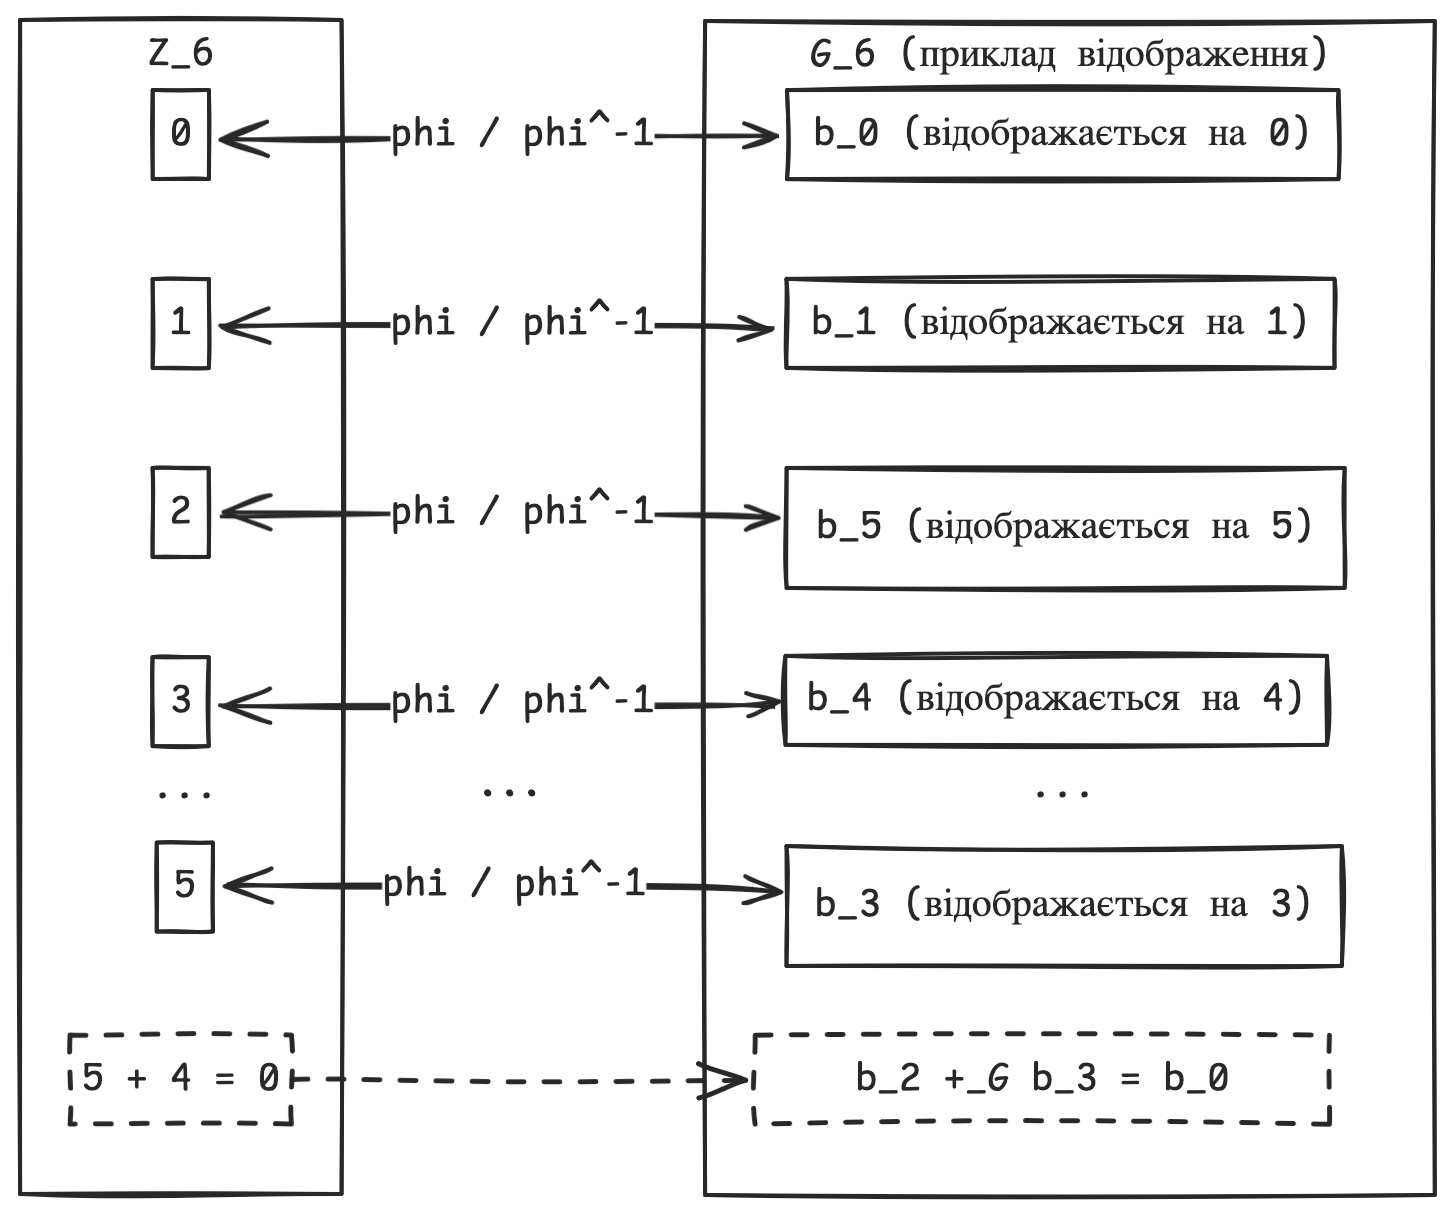
\includegraphics[width=0.5\textwidth]{pictures/G_k vs Z_k Isomorphism Example}
    \caption{Візуалізація ізоморфізму $\varphi$ між $Z_k$ та $G_k$ та відповідності операцій.}
    \label{fig:gk_zk_iso}
\end{figure}

\subsection{Сюр'єкції кілець ($\psi, \lambda$) та фактор-множини}
\label{subsec:ring_surjection}
Окрім ізоморфізмів, протокол використовує сюр'єктивні гомоморфізми (сюр'єкції), означення яких наведено у~\ref{subsec:ring_mappings}.
Ці відображення проектують інформацію з більшого кільця $G_k$ на менше робоче кільце $G_m$.
Архітектура протоколу (див. рис.~\ref{fig:schema}) містить дві такі сюр'єкції: $\psi: G_k \to G_m$ та $\lambda: G_k \to G_m$.
Для їх природного означення $k$ зазвичай вибирається кратним $m$, тобто $k=lm$.
Типовим прикладом є природне відображення $\pi: Z_k \to Z_m$, де $\pi(\bar{a} \bmod k) = \overline{a \bmod m}$, що є гомоморфізмом кілець при $m|k$.

Кожній сюр'єкції $\psi: G_k \to G_m$ відповідає її ядро $\ker \psi = \{x \in G_k \mid \psi(x) = 0_G\}$, яке є ідеалом у $G_k$.
Фактор-множина $G_k/\psi$ (точніше, фактор-кільце $G_k/\ker \psi$) складається з класів суміжності ядра, тобто множин вигляду $x + \ker \psi = \{x+y \mid y \in \ker \psi\}$ для $x \in G_k$.
Як зазначено у~\ref{subsec:factor_rings}, перша теорема про ізоморфізм гарантує, що $G_k/\ker \psi \cong \mathrm{Im}(\psi)$.
Оскільки $\psi$ сюр'єктивне на $G_m$, маємо $G_k/\ker \psi \cong G_m$.

Протокол використовує фактор-множини $G_k/\psi$ та $G_k/\lambda$ як множини прообразів.
Кожному елементу $y \in G_m$ відповідає унікальний клас (елемент фактор-множини), тобто множина $\psi^{-1}(y) = \{x \in G_k \mid \psi(x) = y\}$.
Далі вводяться бієкції $\psi_1: G_k/\psi \to G_m$ та $\lambda_1: G_k/\lambda \to G_m$, які формалізують зв'язок між класами фактор-множини та елементами цільового кільця $G_m$.
Їхня роль полягає в обфускації: значення $y \in G_m$ (або його еквівалент у $Z_m$) публічно представляється не самим $y$, а вибором елемента $x$ з більшого кільця $G_k$, що належить до відповідного класу прообразу ($\psi(x) = y$).
Наприклад, коли Аліса публікує коефіцієнти системи або Боб передає компоненти шифрограми, значення, обчислені у $G_m$ (або $Z_m$), відображаються через $\psi_1$ чи $\lambda_1$ для ідентифікації відповідного класу у $G_k/\psi$ чи $G_k/\lambda$, а потім з цього класу вибирається представник для передачі.
Це приховує справжнє значення $y$ серед великої множини елементів $G_k$, що суттєво ускладнює аналіз для атакуючого, який не знає конкретних сюр\'єкцій $\psi, \lambda$ та бієкцій $\psi_1, \lambda_1$.
Вибір представника у класі може здійснюватися за певним правилом або випадково, що потенційно підвищує стійкість системи.

На рисунку~\ref{fig:obfuscation_flow} показано приклад потоку даних для обфускації та де-обфускації значень.
\begin{figure}[ht]
    \centering
    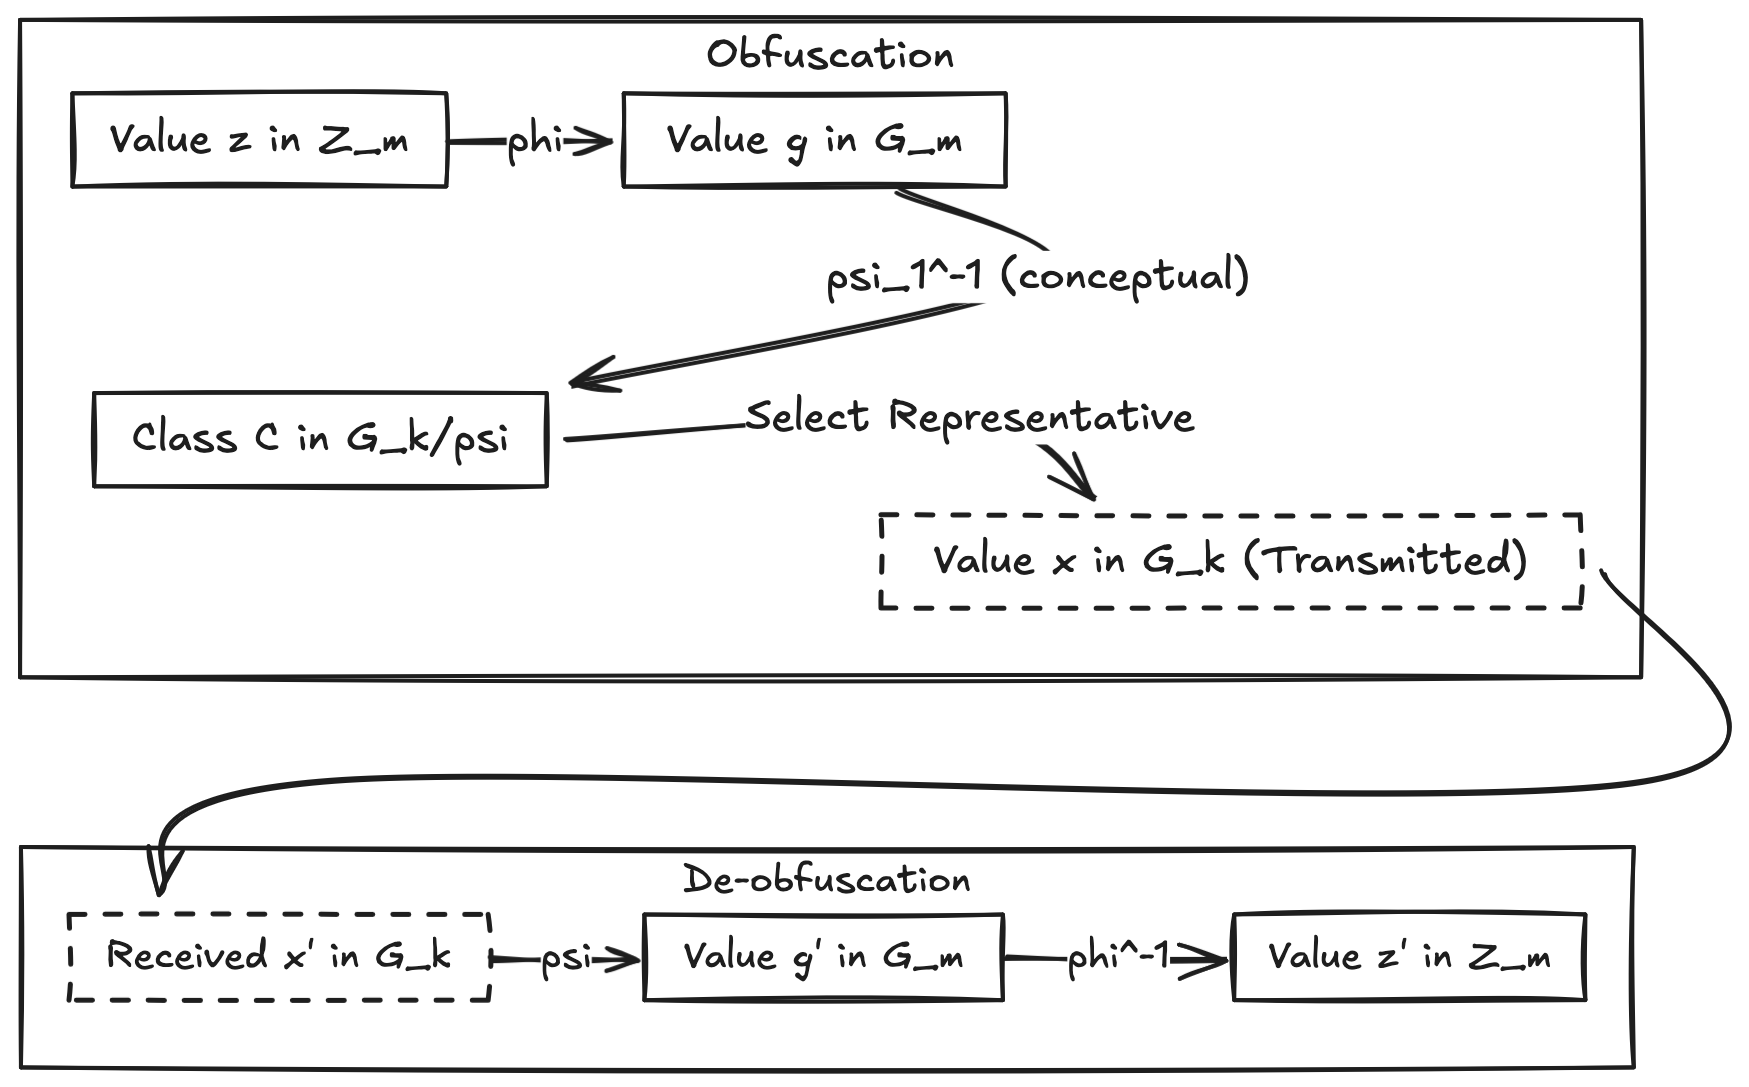
\includegraphics[width=0.9\textwidth]{pictures/De-obfuscation Data Flow Example}
    \caption{Потік даних для обфускації та де-обфускації значення.}
    \label{fig:obfuscation_flow}
\end{figure}

\section{Системи лінійних рівнянь над скінченними кільцями}
\label{sec:sle_over_rings}
Системи лінійних рівнянь (СЛР), визначені над скінченними комутативними кільцями, зокрема над кільцем лишків $Z_m$, є центральним обчислювальним механізмом запропонованої криптосистеми.
Їх властивості, критерії розв'язності та маніпуляції за допомогою матричної алгебри є фундаментальними як для процесу шифрування, так і для дешифрування.
У цьому підрозділі розширюється введення, подане у~\ref{sec:sle_theory}, зосереджуючись на аспектах, що мають безпосереднє відношення до реалізації протоколу.

\subsection{Означення та матричне представлення}
\label{subsec:sle_definition_rings}
Система лінійних рівнянь над $Z_m$ складається з $p$ лінійних конгруенцій відносно $q$ невідомих $x_1, \ldots, x_q$, які мають вигляд:
\[
    \begin{cases}
        a_{11}x_1 + a_{12}x_2 + \cdots + a_{1q}x_q \equiv b_1 \pmod{m} \\
        a_{21}x_1 + a_{22}x_2 + \cdots + a_{2q}x_q \equiv b_2 \pmod{m} \\
        \qquad \vdots \\
        a_{p1}x_1 + a_{p2}x_2 + \cdots + a_{pq}x_q \equiv b_p \pmod{m}
    \end{cases}
\]
Усі коефіцієнти $a_{ij}$, константи $b_i$ та змінні $x_j$ належать кільцю $Z_m = \{\bar{0}, \bar{1}, \ldots, \overline{m-1}\}$.
Всі арифметичні операції (додавання, віднімання, множення) виконуються за модулем $m$.

Система компактно записується у матричній формі:
\[
    Ax \equiv b \pmod{m}
\]
де:
\begin{itemize}
    \item $A = (a_{ij})$ — матриця коефіцієнтів розмірності $p \times q$, $a_{ij} \in Z_m$;
    \item $x = (x_j)$ — стовпчиковий вектор змінних розмірності $q \times 1$;
    \item $b = (b_i)$ — стовпчиковий вектор констант розмірності $p \times 1$.
\end{itemize}
У контексті криптосистеми кількість рівнянь $p$ зазвичай відповідає розміру блоку відкритого тексту, а кількість змінних $q$ обирається так, що $q \geq p$.

\subsection{Критерії розв'язності та структура розв'язків}
\label{subsec:sle_solvability_rings}
Вимогою до криптосистеми є побудова початкової СЛР $l(x) = Ax$ так, щоб конгруенція $Ax \equiv b \pmod{m}$ мала хоча б один розв'язок $\bar{x}$ для \emph{будь-якого} вектора $b \in Z_m^p$.
Критерії розв'язності СЛР над $Z_m$ є складнішими, ніж над полями, особливо при складеному $m$, через наявність дільників нуля (див.~\ref{ex:z8_ops}).
Теорія тісно пов'язана з лінійними діофантовими рівняннями (див.~\ref{subsec:diophantine}).

Достатні умови розв'язності для всіх $b$ стосуються структури матриці $A$:
\begin{enumerate}
    \item \textbf{Лінійна незалежність рядків:} Рядки матриці $A$ повинні бути лінійно незалежними за модулем $m$, тобто жоден рядок не виражається через інші з коефіцієнтами з $Z_m$, окрім тривіального випадку.
    \item \textbf{Існування оберненої підматриці:} У $A$ має існувати підматриця розмірності $p \times p$ (наприклад, стовпці з номерами $i_1, \ldots, i_p$), детермінант якої $\det(A_1)$ є дільником одиниці у $Z_m$, тобто $\gcd(\det(A_1), m) = 1$.
\end{enumerate}
Якщо ці умови виконуються, розв'язність для будь-якого $b$ гарантовано.
Оберненість $A_1$ (через $\det(A_1)$ — дільник одиниці) забезпечує існування єдиного розв'язку для квадратної підсистеми $A_1 u \equiv b \pmod{m}$, де $u$ — відповідні змінні.
Загальний розв'язок початкової системи $Ax \equiv b \pmod{m}$ будується так: координати $x_{i_j}$ прирівнюються до компонент $u$, решта — до нуля.

Варто зазначити, що при $q > p$ розв'язок $\bar{x}$ не єдиний; множина всіх розв'язків утворює афінний підпростір $Z_m^q$, що складається з одного часткового розв'язку та всіх розв'язків відповідної однорідної системи $Ax \equiv 0 \pmod{m}$.
Для шифрування достатньо знайти \emph{будь-який} розв'язок $\bar{x}$.

\subsection{Однорідні системи}
\label{subsec:sle_homogeneous}
Система $Ax \equiv b \pmod{m}$ називається \emph{однорідною}, якщо $b = 0$, тобто $Ax \equiv 0 \pmod{m}$.
Розв'язки однорідної системи (яка завжди має тривіальний розв'язок $x \equiv 0$) описують структуру множини розв'язків відповідної неоднорідної системи (будь-які два розв'язки $Ax \equiv b$ відрізняються на розв'язок $Ax \equiv 0$).

Існування нетривіальних розв'язків ($x \not\equiv 0$) залежить від властивостей $A$ та $m$.
Наприклад, для квадратної матриці ($p=q$) нетривіальні розв'язки існують тоді і тільки тоді, коли $\det(A)$ дорівнює нулю або є дільником нуля у $Z_m$.

Однорідні системи використовуються для перевірки лінійної незалежності рядків матриці коефіцієнтів $A$ у початковій системі $l(x)=Ax$.
Рядки $A$ лінійно незалежні за модулем $m$ тоді і тільки тоді, коли єдиним розв'язком транспонованої однорідної системи $A^T y \equiv 0 \pmod{m}$ є тривіальний розв'язок $y \equiv 0$.
Перевірка цієї умови є необхідним кроком при побудові допустимої матриці $A$ для криптосистеми.

\subsection{Матричні операції у $Z_m$}
\label{subsec:matrix_ops_zm}
Всі обчислення з СЛР виконуються стандартними матричними операціями, адаптованими до кільця $Z_m$.
Додавання та віднімання матриць здійснюється покомпонентно за модулем $m$.
Множення матриць виконується за стандартним правилом ``рядок на стовпець'' з приведенням усіх проміжних результатів за модулем $m$.

Обернення матриць є особливо важливою операцією у протоколі.
Воно необхідне для дешифрування (Аліса обчислює $B_i^{-1}$ для секретних матриць перетворення) та, можливо, для знаходження розв'язку $\bar{x}$ при шифруванні (якщо Боб використовує обернену підматрицю $A_1$).
Квадратна матриця $M \in Z_m^{p \times p}$ є оберненою тоді і тільки тоді, коли її детермінант $\det(M)$ є дільником одиниці у $Z_m$, тобто $\gcd(\det(M), m) = 1$.
Якщо $\det(M)$ дорівнює нулю або є дільником нуля, матриця $M$ не обернена у $Z_m$.

Якщо $\det(M)$ — дільник одиниці, обернена матриця $M^{-1}$ існує і єдина.
Її можна обчислити такими методами:
\begin{itemize}
    \item \textbf{Метод прискореної матриці (ад'юнкт-метод):} $M^{-1} \equiv (\det(M))^{-1} \cdot \mathrm{adj}(M) \pmod{m}$, де $(\det(M))^{-1}$ знаходиться за допомогою розширеного алгоритму Евкліда, а $\mathrm{adj}(M)$ — ад'юнкт-матриця.
    \item \textbf{Метод Гаусса:} Модифікований метод Гаусса застосовується до $Z_m$, причому ділення на ведучий елемент замінюється множенням на його обернений у $Z_m$.
    Якщо ведучий елемент — дільник нуля або нуль, стандартний алгоритм не застосовується і потребує модифікацій (наприклад, використання нормальної форми Сміта).
\end{itemize}
З огляду на потенційні складнощі матричних операцій, особливо обернення, у $Z_m$ при складеному $m$, доцільно використовувати ізоморфізм $\varphi: G_m \to Z_m$.
Відображуючи елементи матриць з $G_m$ у $Z_m$, всі обчислення виконуються у стандартному кільці $Z_m$ із застосуванням ефективних алгоритмів (наприклад, розширеного алгоритму Евкліда для знаходження обернених).
Отримані результати за потреби повертаються у $G_m$ через $\varphi$.
Такий підхід суттєво підвищує ефективність обчислень і спрощує реалізацію.


\section{Основний криптографічний механізм}
\label{sec:core_mechanism}
Після викладення необхідних відомостей про скінченні кільця, відображення та системи лінійних рівнянь над цими кільцями, синтезуємо ці елементи для опису основного криптографічного механізму запропонованого протоколу.
Цей механізм поєднує базову лінійну систему $l(x)$ та секретне афінне перетворення $L(x)$, а також обфускацію за допомогою ізоморфізмів і сюр'єкцій кілець для забезпечення стійкого шифрування та дешифрування.
У цьому підрозділі викладаються фундаментальні принципи цих операцій, а конкретні інтерактивні кроки між Алісою і Бобом розглядаються у Розділі~3.

\subsection{Шифрування через перетворення та обчислення СЛР}
\label{subsec:encryption_mechanism}
Основна ідея шифрування полягає у кодуванні блоку відкритого тексту $v$, представленого вектором у $Z_m^p$, за допомогою двох пов'язаних систем лінійних рівнянь $l(x)$ та $L(x)$, обчислених у спеціально вибраних точках.
Процес складається з кількох концептуальних етапів:

\begin{enumerate}
    \item \textbf{Визначення базової системи ($l(x)$):} Початково визначається базова лінійна система $l(x) = Ax$, де $A$ — матриця розмірності $p \times q$ з елементами у $G_m$ (або її еквівалент $\hat{A}$ у $Z_m$).
    Як зазначено у~\ref{subsec:sle_solvability_rings}, матриця $A$ має бути побудована так, щоб система $Ax \equiv b \pmod{m}$ була розв'язною для будь-якого вектора $b \in G_m^p$.
    Це передбачає лінійну незалежність рядків $A$ та існування оберненої підматриці розмірності $p \times p$.

    \item \textbf{Секретне афінне перетворення ($l(x) \to L(x)$):} Далі застосовується послідовність секретних афінних перетворень до базової системи $l(x)$:
    \[
        L(x) = B_r(B_{r-1}(\ldots B_2(B_1(l(x)+a_1)+a_2)\ldots + a_{r-1})+a_r)+a_{r+1}
    \]
    Тут $B_1, \ldots, B_r$ — секретні обернені матриці розмірності $p \times p$ у $G_m$, а $a_1, \ldots, a_{r+1}$ — секретні вектори розмірності $p \times 1$.
    Позначимо $D = B_r B_{r-1} \ldots B_1$ — загальна лінійна частина перетворення (також обернена).
    В результаті $L(x)$ має загальний афінний вигляд $L(x) = Bx + a$, де $B$ та $a$ залежать від $A$, $B_i$ та $a_j$.
    Послідовність $(B_i, a_j)$ є секретною.
    Всі обчислення виконуються у $G_m$ або, еквівалентно, у $Z_m$ через ізоморфізм $\varphi$.

    \item \textbf{Обчислення шифротексту:} Для шифрування конкретного блоку $v \in Z_m^p$ сторона, що шифрує (Боб), виконує такі дії, працюючи з представленнями у $Z_m$:
    \begin{itemize}
        \item \textbf{Знаходження розв'язку для відкритого тексту ($\bar{x}$):} Боб розв'язує базову систему для заданого $v$, знаходячи вектор $\bar{x} \in Z_m^q$ такий, що $\hat{l}(\bar{x}) = \hat{A}\bar{x} \equiv v \pmod{m}$.
        Оскільки $q \geq p$ і $A$ побудовано відповідно, розв'язок існує.
        Якщо розв'язків декілька, обирається будь-який.
        \item \textbf{Вибір випадкового вектора ($\bar{a}$):} Боб генерує новий випадковий вектор $\bar{a} \in Z_m^q$, незалежно для кожного блоку.
        \item \textbf{Обчислення компонент шифротексту ($d, d_1$):} Боб обчислює два вектори у $Z_m^p$:
        \begin{itemize}
            \item $d = \hat{l}(\bar{a}) = \hat{A}\bar{a} \pmod{m}$ — результат застосування базового лінійного відображення до випадкового вектора.
            \item $d_1 = \hat{L}(\bar{x} + \bar{a}) = \hat{B}(\bar{x} + \bar{a}) + \hat{a} \pmod{m}$ — результат застосування афінного перетворення до суми розв'язку та випадкового вектора.
        \end{itemize}
    \end{itemize}

    \item \textbf{Представлення та передача шифротексту:} Пара векторів $(d, d_1)$ є основною криптографічною інформацією, що представляє зашифрований блок $v$.
    Перед передачею ці вектори (у $Z_m$) обфускуються за допомогою відображень кілець: спочатку відображаються у $G_m$ через $\varphi$, далі — через бієкцію (наприклад, $\psi_1: G_k/\psi \to G_m$) кожна компонента відображається у відповідний клас фактор-множини $G_k/\psi$, після чого з кожного класу вибирається представник у $G_k$ для формування переданих векторів $(\bar{d}, \bar{d}_1)$.
    Така багаторівнева обфускація приховує справжні значення $d$ та $d_1$.
\end{enumerate}

На рисунку~\ref{fig:encryption_logic} наведено концептуальну схему процесу шифрування.
\begin{figure}[ht]
    \centering
    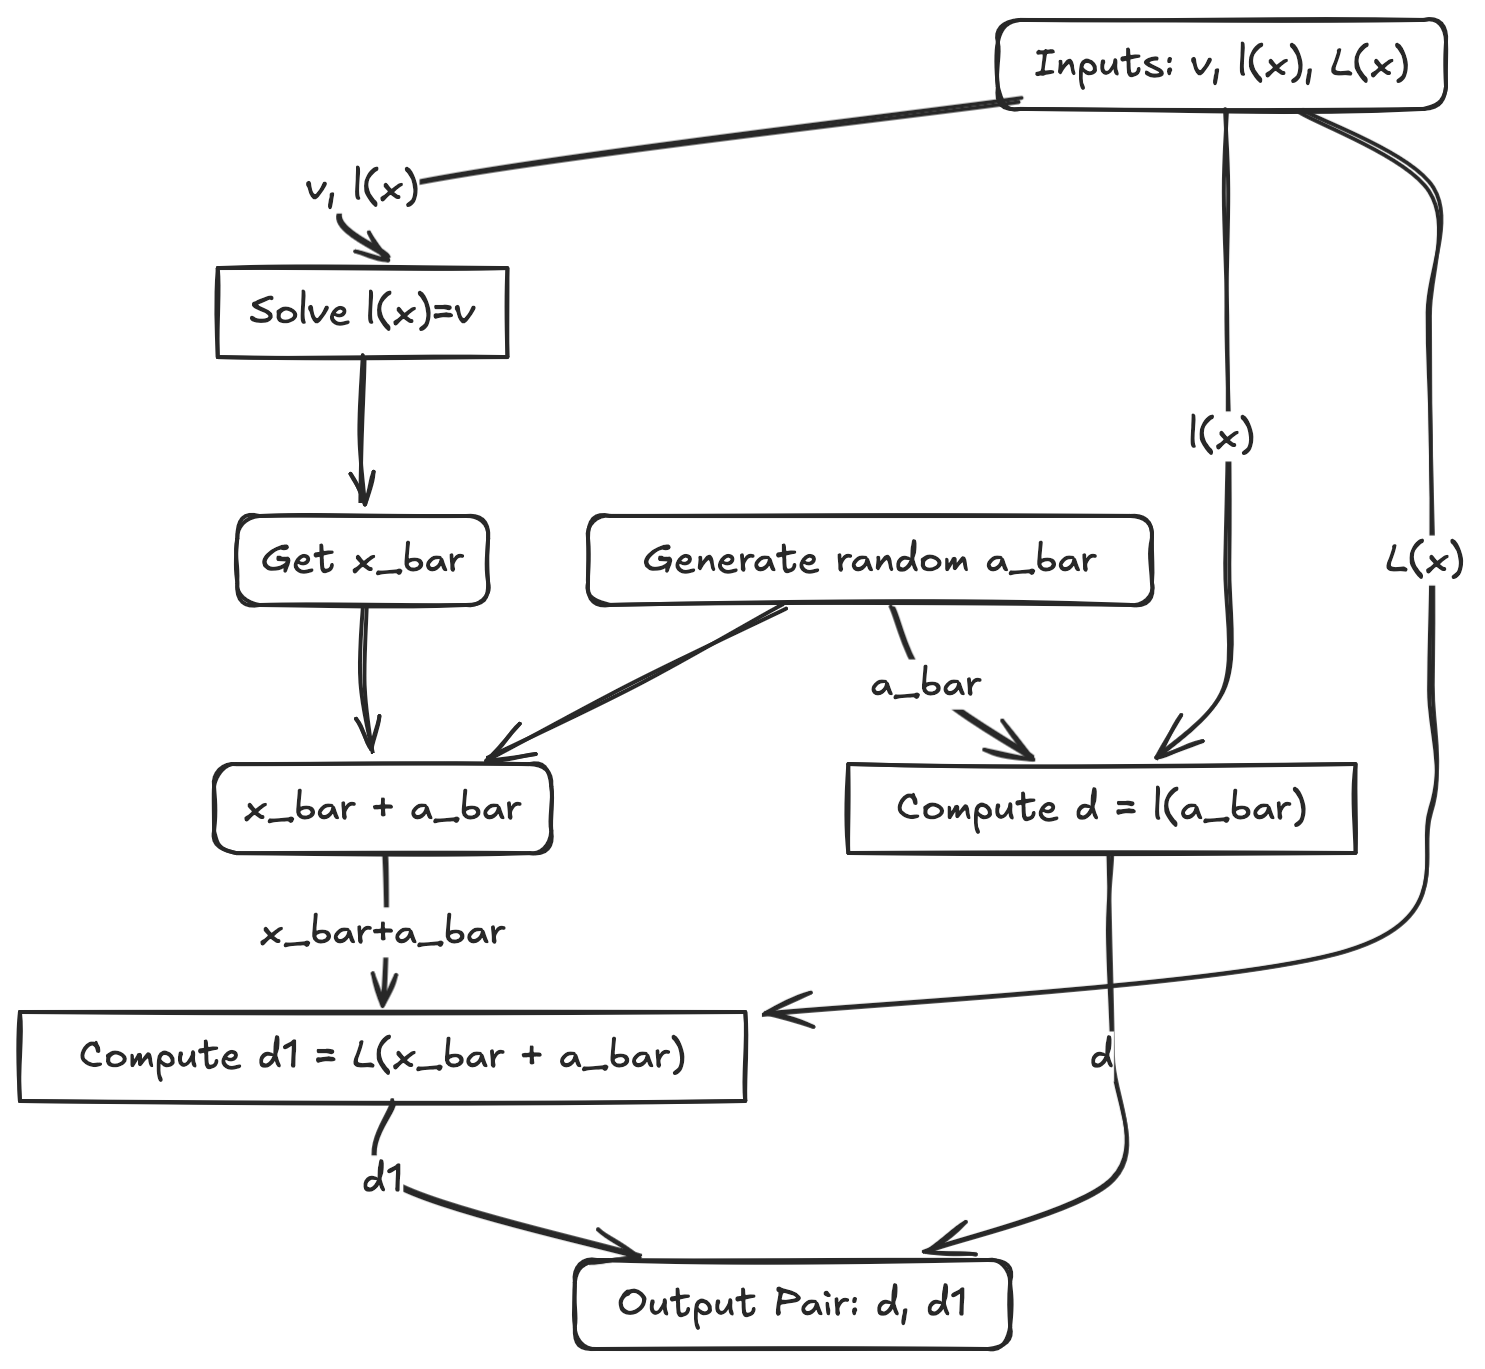
\includegraphics[width=0.5\textheight,keepaspectratio]{pictures/Encryption Core Logic Conceptual Diagram}
    \caption{Концептуальна схема процесу шифрування.}
    \label{fig:encryption_logic}
\end{figure}

\subsection{Дешифрування через зворотні перетворення}
\label{subsec:decryption_mechanism}
Дешифрування виконує сторона (Аліса), яка знає секретні компоненти: відображення ($\varphi, \psi_1$ тощо) та параметри афінного перетворення ($B_i, a_j$).
Процес полягає у зворотному відтворенні кроків шифрування для відновлення відкритого тексту $v$.

\begin{enumerate}
    \item \textbf{Відновлення основних компонент шифротексту ($d, d_1$):} Аліса отримує обфусковану пару $(\bar{d}, \bar{d}_1)$ з елементів $G_k$, застосовує зворотні відображення для отримання векторів $d, d_1$ у $Z_m$.
    Це включає використання зворотної бієкції (наприклад, $\psi_1^{-1}$) та зворотного ізоморфізму $\varphi^{-1}$.

    \item \textbf{Обчислення обернених перетворень:} Аліса обчислює обернені до секретних матриць $B_i$, переводячи їх у $Z_m$ через $\varphi^{-1}$ та знаходячи обернені $\hat{B}_i^{-1}$ у $Z_m$.
    Оскільки $\det(\hat{B}_i)$ — дільник одиниці, обернення можливе (див.~\ref{subsec:matrix_ops_zm}).
    Позначимо $D = B_r \ldots B_1$, тоді $\hat{D}^{-1} = \hat{B}_1^{-1} \ldots \hat{B}_r^{-1}$.

    \item \textbf{Зворотне афінне перетворення:} Аліса, знаючи $\hat{B}_i^{-1}$ та $\hat{a}_j = \varphi^{-1}(a_j)$, алгебраїчно відновлює $\hat{l}(\bar{x} + \bar{a}) + \hat{a}_1$ із $d_1$.
    Якщо $L(y) = D(l(y) + a_1) + c$, то
    \[
        \hat{D}^{-1}(d_1 - \hat{c}) = \hat{l}(\bar{x} + \bar{a}) + \hat{a}_1
    \]
    де $\hat{c}$ — накопичена константа, що залежить від $\hat{a}_2, \ldots, \hat{a}_{r+1}$ та $\hat{B}_i$.

    \item \textbf{Виділення відкритого тексту ($v$):} Аліса використовує $d = \hat{l}(\bar{a})$ та $\hat{a}_1$ для остаточного обчислення:
    \[
        (\hat{l}(\bar{x} + \bar{a}) + \hat{a}_1) - (\hat{l}(\bar{a}) + \hat{a}_1) = \hat{l}(\bar{x})
    \]
    Оскільки $\hat{l}(x)$ — лінійне відображення, $\hat{l}(\bar{x}) = v$, тобто відновлюється початковий блок відкритого тексту.
    Коректність цього процесу випливає з властивостей афінних перетворень та лінійності $l(x)$.
\end{enumerate}

На рисунку~\ref{fig:decryption_logic} наведено концептуальну схему процесу дешифрування.
\begin{figure}[ht]
    \centering
    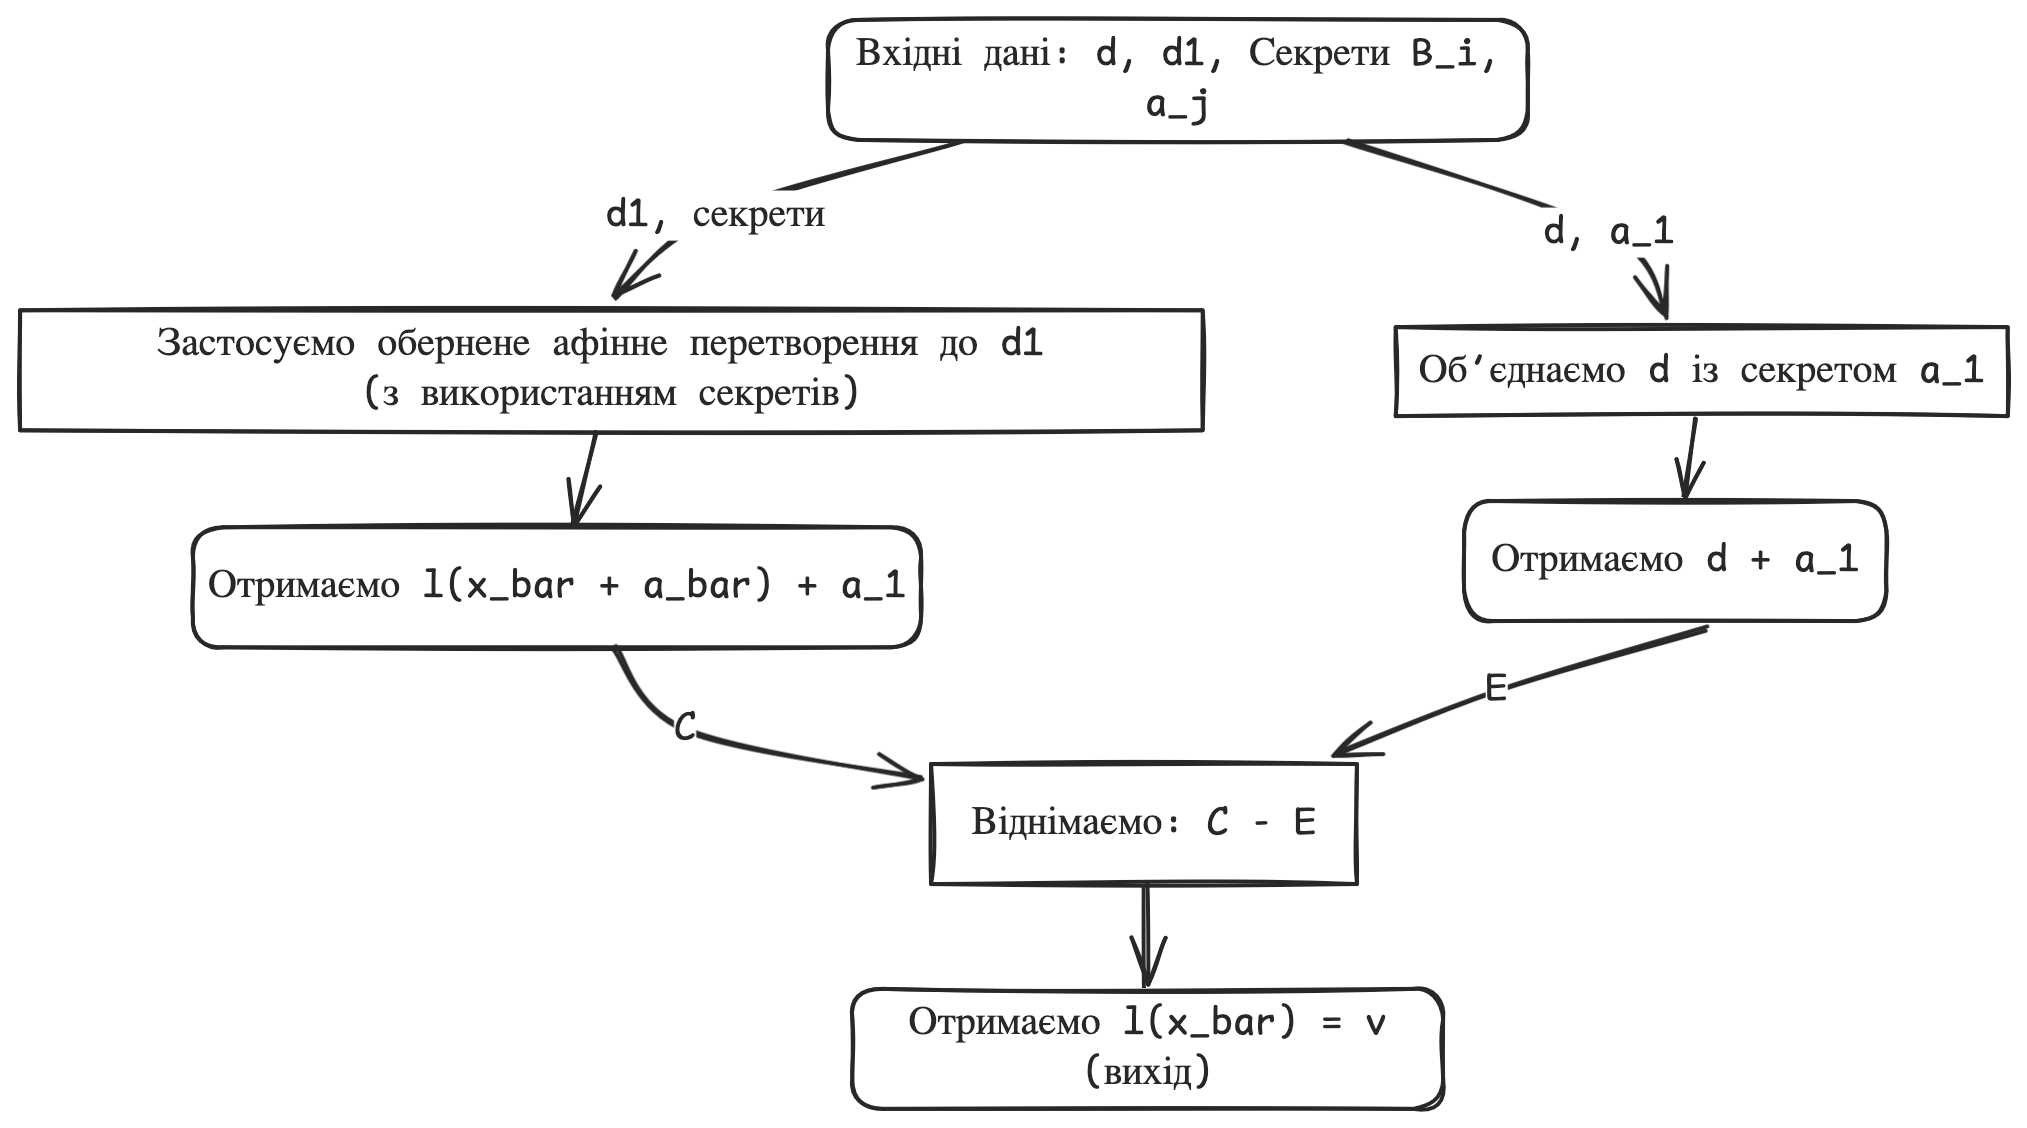
\includegraphics[width=0.9\textwidth]{pictures/Decryption Core Logic Conceptual Diagram}
    \caption{Концептуальна схема процесу дешифрування.}
    \label{fig:decryption_logic}
\end{figure}

\subsection{Роль випадковості та відображень}
\label{subsec:randomness_mappings_role}
Два компоненти є ключовими для стійкості та функціонування механізму, окрім самих перетворень СЛР: випадковий вектор $\bar{a}$ та різноманітні відображення кілець.

Випадковий вектор $\bar{a} \in Z_m^q$, що обирається Бобом для кожного блоку, відіграє роль, аналогічну до ініціалізаційного вектора у класичних симетричних шифрах, але інтегрований у схему інакше.
Його основна функція — забезпечення ймовірнісного шифрування, тобто семантичної стійкості.
Оскільки обидві компоненти шифротексту $d = \hat{l}(\bar{a})$ та $d_1 = \hat{L}(\bar{x} + \bar{a})$ залежать від $\bar{a}$, шифрування одного й того ж блоку $v$ у різний час дає статистично незалежні пари $(\bar{d}, \bar{d}_1)$.
Це унеможливлює частотний аналіз.

Відображення кілець ($\varphi, \psi, \lambda, \psi_1, \lambda_1$) виконують декілька функцій:
\begin{itemize}
    \item \textbf{Обчислювальна ефективність ($\varphi$):} Ізоморфізм $\varphi: Z_m \to G_m$ дозволяє виконувати всі складні обчислення (обернення матриць, розв'язання СЛР) у стандартному кільці $Z_m$.
    \item \textbf{Структурна обфускація ($G_m$):} Використання $G_m$ замість $Z_m$ приховує структуру модульної арифметики, ускладнюючи застосування класичних атак без знання ізоморфізму $\varphi$.
    \item \textbf{Обфускація представлення ($\psi, \lambda, \psi_1, \lambda_1$):} Сюр'єкції та бієкції фактор-множин дозволяють представляти значення з $Z_m$ або $G_m$ зовнішньо як елементи з більшого кільця $G_k$, приховуючи справжню структуру та значення $d, d_1$.
    Для атакуючого, що спостерігає $\bar{d}, \bar{d}_1$ у $G_k$, відновлення $d, d_1$ у $Z_m$ вимагає знання секретних відображень.
\end{itemize}
У сукупності ці відображення створюють багаторівневий захист, що вимагає від атакуючого розкриття кількох структурних секретів, окрім вирішення основної алгебраїчної задачі для перетворених СЛР.


\section{Архітектура системи та генерація компонентів}
\label{sec:architecture_generation}
Після детального розгляду основних алгебраїчних структур, відображень і криптографічного механізму, переходимо до загальної архітектури системи та процесу генерації її ключових компонентів.
Практична реалізація криптосистеми ґрунтується на детермінованому методі побудови необхідних кілець і відображень із набору спільних секретних параметрів, що гарантує узгодженість алгебраїчного середовища для обох абонентів, навіть якщо воно є обфускованим.

\subsection{Схематичний огляд системи}
\label{subsec:system_diagram}
Концептуальна архітектура криптосистеми зображена на рис.~\ref{fig:schema}.

\begin{figure}[ht]
  \centering
  \begin{tikzpicture}[node distance=1.5cm and 2.5cm, >=latex]
    % Define Nodes
    \node (Zm)                  {\(Z_m\)};
    \node (Gm_top) [right=of Zm, yshift=1.5cm] {\(G_m\)};
    \node (Gm_bot) [right=of Zm, yshift=-1.5cm]{\(G_m\)};
    \node (Gk)     [right=of Gm_top, xshift=1cm, yshift=-1.5cm] {\(G_k\)};
    \node (Gk_psi) [above=of Gk] {\(G_k/\psi\)};
    \node (Gk_lam) [below=of Gk] {\(G_k/\lambda\)};

    % Z_m <-> G_m (top)
    \draw[->] (Zm) -- node[above, sloped] {\(\varphi\)} (Gm_top);
    \draw[->] (Gm_top) -- node[below, sloped] {} (Zm);

    % Z_m <-> G_m (bottom)
    \draw[->] (Zm) -- node[below, sloped] {\(\varphi\)} (Gm_bot);
    \draw[->] (Gm_bot) -- node[above, sloped] {} (Zm);

    % G_k -> G_m (top & bottom)
    \draw[->] (Gk) -- node[above, sloped] {\(\psi\)} (Gm_top);
    \draw[->] (Gk) -- node[below, sloped] {\(\lambda\)} (Gm_bot);

    % G_k -> G_k factor rings
    \draw[->] (Gk) -- (Gk_psi);
    \draw[->] (Gk) -- (Gk_lam);

    % Factor rings -> G_m
    \draw[->] (Gk_psi) -- node[above] {\(\psi_1\)} (Gm_top);
    \draw[->] (Gm_top) -- node[below] {} (Gk_psi);

    \draw[->] (Gk_lam) -- node[below] {\(\lambda_1\)} (Gm_bot);
    \draw[->] (Gm_bot) -- node[above] {} (Gk_lam);

  \end{tikzpicture}
  \caption{Схема системи}
  \label{fig:schema}
\end{figure}

Ця схема ілюструє взаємозв'язки та можливі потоки даних між різними алгебраїчними компонентами:
\begin{itemize}
    \item \textbf{$Z_m$}: Стандартне кільце лишків за модулем $m$. Основна роль — домен для ефективних обчислень, зокрема для матричних операцій (обернення, розв'язання СЛР).
    \item \textbf{$G_m$}: Робоче кільце, ізоморфне $Z_m$ через $\varphi$. У цьому кільці концептуально визначаються та маніпулюються системи $l(x)$ і $L(x)$. Використання $G_m$ забезпечує структурну обфускацію, оскільки його представлення залежить від секретного визначального рядка.
    \item \textbf{$G_k$}: Більше кільце, ізоморфне $Z_k$ ($k=lm$), використовується переважно як джерело для обфускованих представлень значень, що походять з $G_m$ або $Z_m$.
    \item \textbf{$\psi, \lambda$}: Дві різні сюр'єктивні гомоморфізми кілець, що відображають елементи з $G_k$ у робоче кільце $G_m$. Вони визначають зв'язок між простором представлення $G_k$ та обчислювальним простором $G_m$.
    \item \textbf{$G_k/\psi, G_k/\lambda$}: Фактор-множини (класи суміжності), породжені сюр'єкціями $\psi$ та $\lambda$. Кожен елемент у $G_k/\psi$ (або $G_k/\lambda$) — це підмножина $G_k$, що містить усі елементи, які відображаються у той самий елемент $G_m$ через $\psi$ (або $\lambda$). Ці фактор-множини слугують проміжними структурами для зовнішнього представлення даних.
    \item \textbf{$\psi_1, \lambda_1$}: Бієкції, що встановлюють взаємно однозначну відповідність між фактор-множинами $G_k/\psi$ (або $G_k/\lambda$) та кільцем $G_m$. Вони забезпечують механізм переходу між елементом у $G_m$ та відповідним класом прообразу, дозволяючи вибирати представників із $G_k$ для зовнішньої комунікації.
    \item \textbf{$\varphi$}: Ключовий ізоморфізм, що пов'язує $G_m$ та $Z_m$, забезпечуючи перехід між потенційно обфускованим робочим кільцем $G_m$ та ефективним обчислювальним кільцем $Z_m$.
\end{itemize}
Архітектура підтримує декілька шляхів представлення та обробки даних. Наприклад, у типовому варіанті протоколу: Аліса визначає $l(x)$ і $L(x)$ у $G_m$, відображає їх коефіцієнти через $\lambda_1$ у $G_k/\lambda$, публікує представників із $G_k$. Боб отримує ці дані, повертає їх через $\lambda_1^{-1}$ у $G_m$, далі через $\varphi^{-1}$ у $Z_m$ для отримання $\hat{l}(x), \hat{L}(x)$ для обчислень. Боб обчислює компоненти шифротексту $d, d_1$ у $Z_m$, відображає їх через $\varphi$ у $G_m$, далі через $\psi_1$ у $G_k/\psi$ і передає представників із $G_k$. Аліса виконує зворотне відображення через $\psi_1^{-1}$ та $\varphi^{-1}$ для отримання $d, d_1$ у $Z_m$ для дешифрування. Такий багаторівневий підхід із залученням кількох кілець і відображень спрямований на обфускацію обчислень і даних від зовнішніх спостерігачів.

\subsection{Генерація кілець і відображень (алгоритм GEN-G)}
\label{subsec:gen_g_algorithm}
Конкретні екземпляри ізоморфних кілець $G_k$ і $G_m$, а також ключовий ізоморфізм $\varphi: Z_m \to G_m$, не вибираються довільно, а генеруються детерміновано з набору спільних секретних параметрів за допомогою алгоритму GEN-G.

\textbf{Алгоритм GEN-G$(a,c,l,k)$:}
\begin{itemize}
    \item \textbf{Вхід:} Набір секретних цілих параметрів $(a, c, l, k)$. Тут $k$ — порядок більшого кільця $G_k$, $m$ ($k=lm$) — порядок робочого кільця $G_m$, а $a, c$ — коефіцієнти лінійної конгруентної функції $f(i) = a \cdot i + c$. Важливою умовою є $\gcd(a, k) = 1$, що гарантує, що при пробіганні $i$ по повній системі лишків за модулем $k$, значення $a \cdot i + c \pmod{k}$ також утворюють повну систему лишків, тобто перестановку.
    \item \textbf{Вихід:} Визначальний рядок $b = (b_1, b_2, \ldots, b_k)$ для кільця $G_k$, який неявно визначає його структуру та ізоморфізм із $Z_k$.
    \item \textbf{Метод:} Алгоритм складається з кількох послідовних кроків:
    \begin{enumerate}
        \item \textbf{Генерація початкового рядка:} Створюється масив $b'$ довжини $k$ за лінійною конгруентною функцією:
        \[
            \text{for } i = 0 \text{ to } k-1 \text{ do } b'[i+1] := (a \cdot i + c) \pmod{k}
        \]
        Оскільки $\gcd(a,k)=1$, масив $b'$ є перестановкою елементів $\{0, 1, \ldots, k-1\}$.
        \item \textbf{Секретне перетворення:} Початковий рядок $b'$ трансформується згідно з набором заздалегідь погоджених секретних правил, відомих лише Алісі та Бобу. Ці правила визначають послідовність перестановок або інших модифікацій масиву (наприклад, обмін сусідніх елементів, циклічні зсуви тощо). Конкретна послідовність таких перетворень є частиною секретного ключа і суттєво збільшує кількість можливих визначальних рядків. Обидва абоненти повинні застосовувати ідентичні перетворення у тій самій послідовності.
        \item \textbf{Нормалізація (фіксація 0 та 1):} Трансформований масив нормалізується: елемент зі значенням 1 розміщується на першій позиції, а елемент зі значенням 0 — на останній. Отриманий масив $b = (b_1=1, b_2, \ldots, b_{k-1}, b_k=0)$ є фінальним визначальним рядком, що повністю визначає кільце $G_k$ та ізоморфізм $g: Z_k \to G_k$. Відображення задається як $g(\bar{1}) = b_1 = 1$, $g(\bar{i}) = b_i$ для $i=2, \ldots, k-1$, $g(\bar{0}) = b_k = 0$. Ізоморфізм $\varphi: Z_m \to G_m$, необхідний для протоколу, отримується або запуском цього ж процесу з параметрами $(a, c, 1, m)$, або відповідним обмеженням/адаптацією $g$ для $G_m$.
        \item \textbf{Генерація відображення наступника (опціонально):} З фінального визначального рядка $b$ будується допоміжний масив $P[0 \ldots k-1]$, що реалізує операцію "додати одиницю" у $G_k$: $P[0] := b_1 (=1)$; $P[b_i] := b_{i+1}$ для $i=1, \ldots, k-2$; $P[b_{k-1}] := b_k (=0)$. Це відображення може використовуватись для побудови повних таблиць операцій у $G_k$, але на практиці достатньо ізоморфізму $\varphi$ для ефективних обчислень у $Z_m$.
    \end{enumerate}
\end{itemize}
Правильність алгоритму ґрунтується на тому, що лінійна конгруентна функція породжує перестановку при $\gcd(a,k)=1$ (див.~\ref{subsec:residue_rings}).
Обчислювальна складність визначається $k$ операціями множення за модулем, тобто $O(k \log^2 k)$, що є прийнятним для відносно невеликих $k$.

Важливо підкреслити, що алгоритм GEN-G генерує лише кільця $G_k, G_m$ та ізоморфізм $\varphi$.
Інші критично важливі секретні компоненти криптосистеми — конкретні сюр'єкції $\psi, \lambda$, відповідні бієкції $\psi_1, \lambda_1$, а також параметри секретних афінних перетворень $B_i, a_j$ — мають бути погоджені окремо між Алісою та Бобом через захищений канал або виведені з початкових секретів за додатковою домовленістю.
Ці додаткові компоненти завершують повну специфікацію спільного симетричного ключа.


\section{Теоретичні аспекти стійкості}
\label{sec:theoretical_security}
Стійкість запропонованої симетричної криптосистеми, як і будь-якої криптографічної схеми, ґрунтується на припущенні про обчислювальну складність певних базових математичних задач для супротивника, який має доступ лише до публічної інформації (наприклад, відкритих систем $\bar{l}(x), \bar{L}(x)$ та перехоплених шифротекстів $(\bar{d}, \bar{d}_1)$), але не володіє спільними секретними компонентами ключа.
Сила системи зумовлена поєднанням факторів, пов'язаних із комбінаторною складністю визначення секретних відображень між кільцями та труднощами зворотного відтворення секретних алгебраїчних перетворень, застосованих до систем лінійних рівнянь.

\subsection{Складність визначення ізоморфізмів та відображень}
\label{subsec:hardness_mappings}
Вагома частина стійкості системи забезпечується обфускацією, яку створюють нестандартні представлення кілець ($G_m, G_k$) та відображення між ними ($\varphi, \psi, \lambda, \psi_1, \lambda_1$).
Атакуючий, що намагається зламати систему, повинен спочатку (або паралельно) визначити ці секретні структури та відображення.

\begin{itemize}
    \item \textbf{Визначення ізоморфізму $\varphi$:} Ізоморфізм $\varphi: Z_m \to G_m$ задається визначальним рядком $b = (1, b_2, \ldots, b_{m-1}, 0)$, згенерованим алгоритмом GEN-G (див.~\ref{subsec:gen_g_algorithm}). Без знання секретних параметрів $(a, c)$ і, головне, секретних правил перетворення на відповідному кроці GEN-G, атакуючий стикається із задачею відновлення правильної перестановки $b_2, \ldots, b_{m-1}$ елементів $\{2, 3, \ldots, m-1\}$. Кількість таких перестановок становить $(m-2)!$. Додатково, секретні перетворення означають, що отриманий визначальний рядок може не відповідати жодній послідовності, згенерованій лише початковою лінійною конгруентною функцією. Це робить повний перебір ізоморфізмів обчислювально нездійсненним, оскільки простір пошуку зростає факторіально з $m$.
    \item \textbf{Визначення сюр'єкцій та фактор-множин ($\psi, \lambda, \psi_1, \lambda_1$):} Атакуючий також має визначити конкретні сюр'єктивні гомоморфізми $\psi, \lambda: G_k \to G_m$ та відповідні бієкції $\psi_1, \lambda_1$, що пов'язують фактор-множини $G_k/\psi, G_k/\lambda$ з $G_m$. Знаходження конкретного гомоморфізму між двома кільцями — загалом складна задача. У цьому випадку атакуючий повинен визначити правильне відображення з $G_k$ (структура якого вже прихована власним ізоморфізмом $\varphi_k$) на $G_m$ (структура якого прихована $\varphi$). Кількість можливих сюр'єктивних гомоморфізмів залежить від структури кілець та їх ідеалів. Для розбиття $k$ елементів $G_k$ на $m$ непорожніх підмножин (прообрази або класи суміжності), кожна з яких відображається у унікальний елемент $G_m$, кількість варіантів оцінюється як $O(k! / (m! (l!)^m))$, де $l = k/m$. Для $k=50, m=25, l=2$ це $\frac{50!}{25!(2!)^{25}}$, що є надзвичайно великим числом.
\end{itemize}

У сукупності ці фактори дають нижню межу складності повного перебору для відновлення всіх відображень навіть для відносно невеликих порядків кілець. Ця комбінаторна складність є основною лінією захисту.

\subsection{Стійкість, що випливає з перетворень СЛР}
\label{subsec:security_sle_transform}
Окрім складності визначення структур кілець і відображень, додатковий рівень стійкості забезпечується секретним афінним перетворенням, застосованим до систем лінійних рівнянь.
Розглянемо сильну модель атакуючого, який, припустимо, зумів визначити кільця $G_m, G_k$ та всі відповідні відображення ($\varphi, \psi, \lambda, \psi_1, \lambda_1$).
Тобто атакуючий може перевести відкриті системи $\bar{l}(x), \bar{L}(x)$ та перехоплені шифротексти $(\bar{d}, \bar{d}_1)$ у їх еквіваленти $\hat{l}(x), \hat{L}(x)$ та $(d, d_1)$ у стандартному кільці $Z_m$.
Навіть у такому випадку залишаються суттєві перешкоди:

\begin{itemize}
    \item \textbf{Секретність афінного перетворення:} Ядро механізму шифрування — це перетворення $l(x) \to L(x)$, визначене послідовністю секретних обернених матриць $B_i$ та секретних векторів $a_j$.
    Дешифрування вимагає знання цих $B_i$ та $a_j$ для зворотного відтворення, зокрема обчислення та застосування обернених матриць $B_i^{-1}$ і віднімання впливу векторів $a_j$ у правильному порядку (див.~\ref{subsec:decryption_mechanism}). Атакуючий, який знає лише кінцеву афінну систему $\hat{L}(x)$ (і базову $\hat{l}(x)$), але не проміжні кроки ($B_i, a_j$), не може виконати це зворотне перетворення. Задача декомпозиції афінного відображення $\hat{L}(x)$ для відновлення $\hat{l}(x)$ без знання $B_i$ та $a_j$ є обчислювально складною, оскільки існує багато різних послідовностей перетворень, що можуть призвести до одного й того ж $\hat{L}(x)$.
    \item \textbf{Обфускація випадковістю ($\bar{a}$):} Випадковий вектор $\bar{a}$, що обирається для кожного шифрування, ускладнює задачу для атакуючого.
    Він спостерігає $d = \hat{l}(\bar{a})$ та $d_1 = \hat{L}(\bar{x} + \bar{a})$, де $v = \hat{l}(\bar{x})$ — невідомий відкритий текст, $\bar{x}$ — невідомий розв'язок, а $\bar{a}$ — невідомий випадковий вектор.
    Навіть якщо $\hat{l}$ і $\hat{L}$ (тобто $\hat{A}, \hat{B}, \hat{a}$) відомі, атакуючий має лише дві відомі величини ($d, d_1$), пов'язані рівняннями з двома невідомими векторами ($\bar{x}, \bar{a}$) та невідомим $v$.
    Випадковий вектор $\bar{a}$ фактично виконує роль одноразової маски, що приховує зв'язок між $\bar{x}$ (а отже, і $v$) та шифротекстом. Без знання $\bar{a}$ атакуючий не може ізолювати компоненти, пов'язані лише з $\bar{x}$ чи $v$.
\end{itemize}
Отже, навіть якщо структурна обфускація через відображення кілець буде подолана, стійкість системи спирається на складність алгебраїчного зворотного відтворення секретного афінного перетворення $L(x)$ за відомими $l(x)$ і $L(x)$, особливо


\chapter{Приклади лістингів}

У цьому розділі наведено приклади лістингів. Вони наведені суто для прикладу включення таких елементів. 

Перший лістинг.

\lstset{caption={Попередня обробка даних}}
\begin{lstlisting}
#Last column is garbage, so we drop it:
dataset.drop(5409, axis=1, inplace=True)
#Transform our data from string to numbers or Nan:
dataset.iloc[:,:-1] = dataset.iloc[:,:-1].apply(pd.to_numeric, errors='coerce')
#Drop Nan values:
dataset.dropna(inplace=True)
#Change our output to numerical: 'inactive' --> 0 and 'active' --> 1:
dataset.replace({'inactive': 0, 'active': 1}, inplace=True)
\end{lstlisting}
 
Тепер другий лістинг.
\lstset{caption={Підготовка необхідних елементів для аналізу}}
\begin{lstlisting}
#Output column extraction:
test = pd.DataFrame(dataset[5408])

#Computation of correlation of the input columns with output column:
corr_with_res = []

for i in range(5408):
corr_with_res.append((test.join(dataset[i])).astype(float).corr()[5408][i])

whole_corr = pd.DataFrame(corr_with_res)

#Collecting "active" rows:
active = dataset[dataset[5408] == 1]
\end{lstlisting}

І, нарешті, третій. 

\lstset{caption={Функція для здійснення аналізу}}
\begin{lstlisting}
def corr_mean(alpha = 0, beta = 0.4, drop = pd.Index([])):
signif_col = (whole_corr[whole_corr[0].abs() > alpha].index &\\
whole_corr[whole_corr[0].abs() \\
< beta].index).difference(drop)
active_signif = active[signif_col]
active_signif_corr = active_signif.T.astype(float).corr()
mean = 0

for i in range(len(active_signif_corr) - 1):
sum_row_corr = active_signif_corr.iloc[i:i+1,i+1:].T.abs().sum().values[0]
mean += sum_row_corr
mean = mean/(((len(active_signif_corr) - 1)*len(active_signif_corr))/2)
return mean, signif_col
\end{lstlisting}


\chapter{ПРАКТИЧНЕ ПОРІВНЯННЯ ТА РОЗШИРЕННЯ СИСТЕМИ}\label{ch:---:----}

У цьому розділі розглядаються практичні аспекти запропонованої симетричної криптосистеми на основі відображень кілець і систем лінійних рівнянь. Зокрема, наведено порівняння з поширеними симетричними та асиметричними алгоритмами, а також розглянуто потенціал використання протоколу у верифікованому шифруванні та протоколах з нульовим розголошенням. Для ілюстрації продуктивності використано результати тестування референсної (неоптимізованої) реалізації\footnote{Див. \cite{KyrylR24SLE}}.

\section{Порівняння з подібними рішеннями}

\subsection{Загальні характеристики}

Запропонована система суттєво відрізняється від класичних симетричних (AES, ChaCha20) та асиметричних (ElGamal~\cite{ElGamal85}) криптосистем за такими критеріями:

\begin{table}[h!]
\centering
\begin{tabular}{|l|c|c|}
\hline
\textbf{Критерій} & \textbf{SLE} & \textbf{AES-256-GCM}~\cite{NISTSP800-38D, RustCryptoAESGCMDocs} \\
\hline
Тип & Симетрична & Симетрична \\
\hline
Структура ключа & Сукупність параметрів & 256-бітовий ключ \\
\hline
Налаштування & Складне, багатокрокове & Просте \\
\hline
Основа стійкості & Комбінаторика, алгебра & SPN, великий ключ \\
\hline
\end{tabular}
\caption{Порівняння основних характеристик}
\label{tab:table}
\end{table}

\begin{table}[h!]
\centering
\begin{tabular}{|l|c|c|}
\hline
\textbf{Критерій} & \textbf{SLE} & \textbf{ChaCha20Poly1305}~\cite{RFC8439, RustCryptoChaChaPoly1305Docs} \\
\hline
Випадковість & Вбудована & Через nonce \\
\hline
Розширення шифротексту & $\times 2$ & Мінімальне \\
\hline
Продуктивність & Помірна & Висока \\
\hline
\end{tabular}
\caption{Порівняння функціональних властивостей}
\label{tab:table2}
\end{table}

\textbf{Короткі висновки:}
\begin{itemize}
    \item SLE має складніший етап налаштування, але забезпечує великий простір ключів.
    \item Стандартні симетричні алгоритми (AES, ChaCha20) мають просту структуру ключа та надзвичайно високу швидкодію.
    \item SLE забезпечує ймовірнісне шифрування без додаткових режимів, але має розширення шифротексту.
\end{itemize}

\subsection{Порівняння швидкодії}

Нижче наведено результати тестування референсної реалізації SLE (неоптимізованої) у порівнянні з AES-256-GCM та ChaCha20Poly1305 для блоку даних розміром 1024 байти:

\begin{table}[h!]
\centering
\begin{tabular}{|l|c|c|c|}
\hline
\textbf{Алгоритм} & \textbf{SLE} & \textbf{AES-256-GCM}~\cite{NISTSP800-38D, RustCryptoAESGCMDocs} & \textbf{ChaCha20Poly1305}~\cite{RFC8439, RustCryptoChaChaPoly1305Docs} \\
\hline
Encrypt & 985~мкс & 7.25~мкс & 3.99~мкс \\
\hline
\end{tabular}
\caption{Час шифрування (1024 байти)}
\label{tab:table3}
\end{table}

\begin{table}[h!]
\centering
\begin{tabular}{|l|c|c|c|}
\hline
\textbf{Алгоритм} & \textbf{SLE} & \textbf{AES-256-GCM}~\cite{NISTSP800-38D, RustCryptoAESGCMDocs} & \textbf{ChaCha20Poly1305}~\cite{RFC8439, RustCryptoChaChaPoly1305Docs} \\
\hline
Decrypt & 306~мкс & 6.33~мкс & 3.50~мкс \\
\hline
\end{tabular}
\caption{Час дешифрування (1024 байти)}
\label{tab:table4}
\end{table}

\textbf{Висновки:}
\begin{itemize}
    \item SLE суттєво повільніший за сучасні симетричні алгоритми (на 2--3 порядки), що очікувано для прототипної реалізації на основі лінійної алгебри.
    \item Дешифрування у SLE швидше за шифрування, що пов'язано з особливостями протоколу.
    \item Наведені результати отримані для референсної (неоптимізованої) реалізації SLE\footnote{Див. \cite{KyrylR24SLE}}; оптимізація може суттєво покращити продуктивність.
\end{itemize}

\section{Верифіковане шифрування та інтеграція з ZKP}
\label{sec:verifiable_encryption}

\textbf{Верифіковане шифрування} (verifiable encryption) --- це криптографічний підхід, який дозволяє довести правильність певної операції над зашифрованими даними (наприклад, правильність дешифрування, оновлення балансу, чи виконання обчислення) без розкриття секретного ключа чи самих даних.
Такий підхід є ключовим для побудови протоколів з нульовим розголошенням (Zero-Knowledge Proofs, ZKP~\cite{GoldwasserEtAl89, ParnoEtAl13Pinocchio}), приватних транзакцій, а також для побудови довірених обчислень у розподілених системах, схематично представлений на рисунку~\ref{fig:zkp_interaction}.

\begin{figure}[ht]
    \centering
    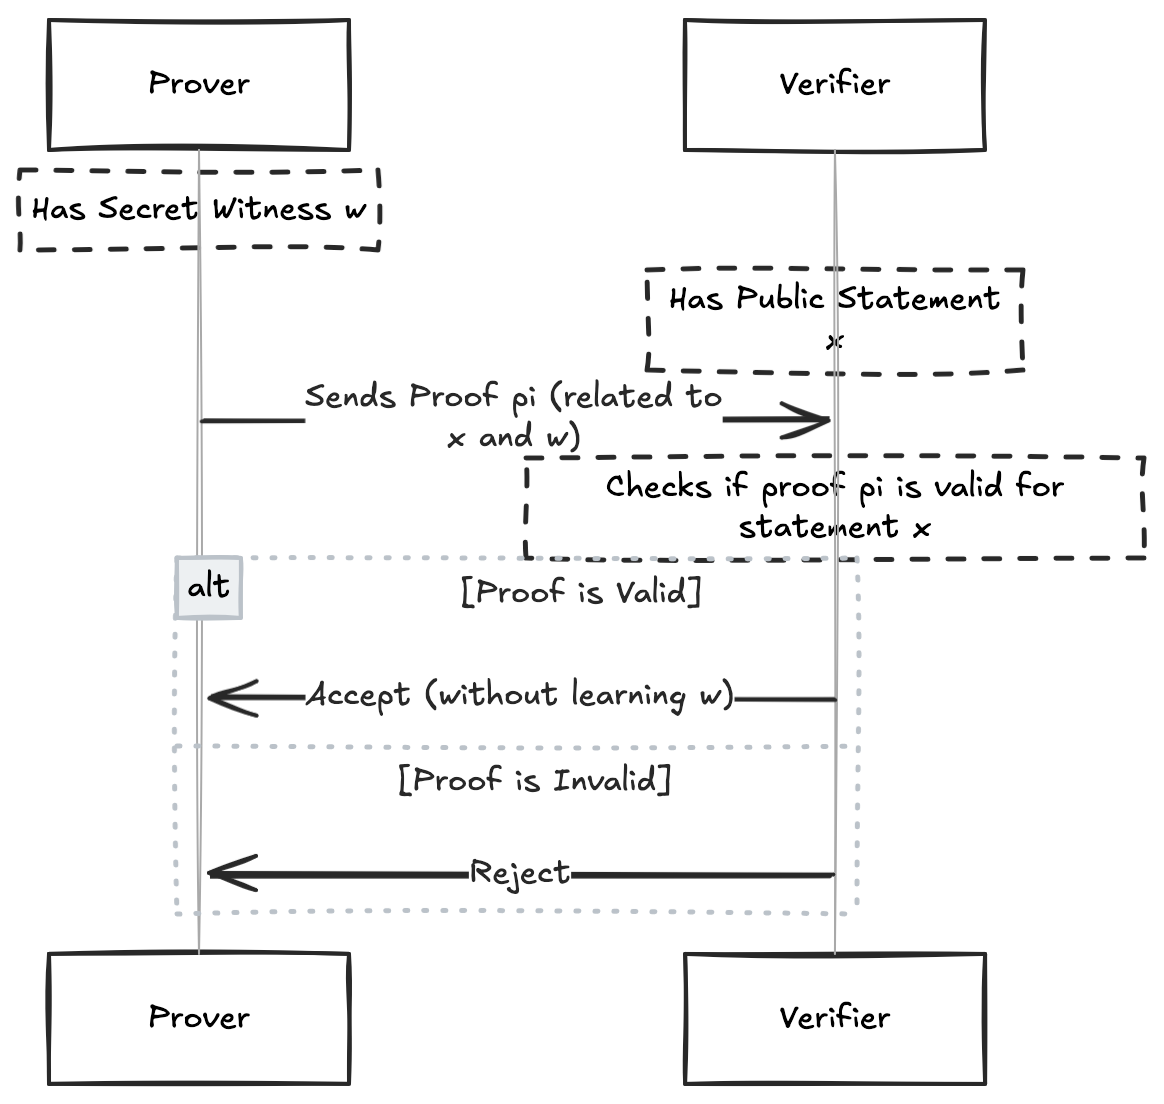
\includegraphics[width=0.4\textheight,keepaspectratio]{pictures/prover-verifier-image}
    \caption{Схематична взаємодія Prover та Verifier у протоколі з нульовим розголошенням.}
    \label{fig:zkp_interaction}
\end{figure}

\textbf{Мотивація:}
\begin{itemize}
    \item Забезпечення приватності: можна довести правильність обробки даних без їх розкриття.
    \item Протидія шахрайству: неможливо підробити доказ без знання секрету.
    \item Використання у блокчейнах, e-voting, приватних платіжних системах.
\end{itemize}

\subsection{SLE-протокол у контексті верифікованого шифрування}\label{subsec:sle-----}

SLE-протокол має алгебраїчну структуру (матричні та векторні операції, розв'язання СЛР), що робить його природним кандидатом для інтеграції з ZKP та верифікованим шифруванням.
Основна ідея полягає у тому, що всі операції протоколу можна виразити у вигляді арифметичних схем (R1CS~\cite{ParnoEtAl13Pinocchio}), які є стандартом для сучасних ZKP-систем (наприклад, zk-SNARK~\cite{Groth16, BenSassonEtAl13}, zk-STARK~\cite{BenSassonEtAl18STARK}).

Серед основних переваг SLE для верифікованого шифрування варто відзначити те, що всі операції протоколу базуються на лінійній алгебрі: робота з векторами та матрицями природно і компактно виражається у вигляді обмежень R1CS, що є стандартом для сучасних ZKP-систем.
Завдяки цьому, для малих розмірностей кількість модульних множень у SLE може бути значно меншою, ніж у схемах на основі піднесення до степеня (наприклад, ElGamal чи RSA), що знижує загальну складність доказу.
Крім того, структурованість лінійної алгебри дозволяє ефективніше оптимізувати схеми у ZKP-фреймворках.

Водночас існують і певні виклики.
По-перше, більшість сучасних ZKP-систем працюють над простими полями, тоді як SLE використовує арифметику у кільці, і емуляція такої арифметики за складеним модулем $m$ може бути обчислювально затратною.
По-друге, якщо відображення у протоколі визначаються великими таблицями, їх ефективне представлення у R1CS є складним; ситуація спрощується лише у випадку, коли відображення мають явну арифметичну формулу.
Нарешті, для складних операцій, таких як обернення матриці, розмір відповідної схеми R1CS може суттєво зрости, що впливає на швидкість генерації та перевірки доказу.

\subsection{Порівняння SLE та ElGamal у контексті ZKP}\label{subsec:-sle--elgamal---zkp}

Типові сценарії застосування верифікованого шифрування включають доведення коректного дешифрування, коли необхідно переконати сторонню особу, що зашифроване повідомлення було правильно розшифроване без розкриття секретного ключа.
Іншим поширеним випадком є доказ оновлення балансу: потрібно підтвердити, що новий шифротекст дійсно відповідає оновленому балансу, не розкриваючи саму суму.
Нарешті, важливим застосуванням є доказ коректного виконання обчислення, коли необхідно довести, що над зашифрованими даними була виконана дозволена операція згідно з протоколом, не розкриваючи вхідні чи проміжні значення.

\textbf{Загальна схема інтеграції SLE з ZKP:}
\begin{enumerate}
    \item Формалізувати операцію (наприклад, дешифрування) як арифметичну схему.
    \item Виразити її у вигляді R1CS (Rank-1 Constraint System~\cite{ParnoEtAl13Pinocchio}).
    \item Згенерувати доказ (наприклад, zk-SNARK~\cite{Groth16, BenSassonEtAl13}) для цієї схеми.
    \item Передати доказ разом із шифротекстом для перевірки.
\end{enumerate}

У схемах на основі піднесення до степеня (ElGamal~\cite{ElGamal85, BonehShoup20}) доведення коректності операцій у ZKP є дорогим через велику кількість мультиплікативних обмежень.
У SLE основні операції — це додавання та множення у кільці, що може бути значно ефективніше для ZKP, особливо для невеликих розмірностей.

SLE-протокол може бути перспективним для застосувань, де потрібне верифіковане шифрування або інтеграція з ZKP, особливо якщо вдасться ефективно реалізувати арифметику у кільці та відображення у сучасних ZKP-фреймворках.
Однак практична ефективність залежить від конкретної реалізації та обмежень обраної ZKP-системи.


\chapter{ВИСНОВКИ}

У роботі запропоновано новий підхід до побудови симетричної криптосистеми, що базується на сюр’єктивних відображеннях між скінченними асоціативно-комутативними кільцями з одиницею та системах лінійних рівнянь над кільцями лишків.

Основною перевагою розробленої системи є можливість використання алгебраїчних структур відносно невеликих порядків без необхідності складних обчислень над великими простими числами чи полями високого порядку.

Запропонований протокол забезпечує багаторівневу обфускацію даних, що підвищує стійкість до криптоаналітичних атак, зокрема перебірних і статистичних.

Стійкість системи ґрунтується на комбінаторній складності множини відображень та ізоморфізмів між кільцями, а також на ймовірнісному характері шифрування, що унеможливлює частотний аналіз.

Практична реалізація алгоритмів у вигляді програмної бібліотеки підтвердила працездатність і ефективність основних ідей.

Розроблена система може бути впроваджена для симетричного шифрування даних у випадках, коли сторони можуть безпечно узгодити спільний ключ, а також у пристроях з обмеженими ресурсами (наприклад, IoT, смарт-картки).

Алгебраїчна структура протоколу створює перспективи для застосування у верифікованих обчисленнях та протоколах з нульовим розголошенням.

Наукова та практична значущість роботи полягає у розвитку напрямів симетричної криптографії на основі нових джерел стійкості, а також у потенціалі для подальшої інтеграції з сучасними технологіями захисту даних.

Подальші дослідження доцільно спрямувати на поглиблений криптоаналіз, оптимізацію продуктивності, розробку рекомендацій щодо вибору параметрів, а також на розширення сфери застосування, зокрема у протоколах верифікованого шифрування та захищених обчислень.

\renewcommand{\bibname}{ПЕРЕЛІК ДЖЕРЕЛ ПОСИЛАННЯ}
\clearpage
\phantomsection
\addcontentsline{toc}{chapter}{ПЕРЕЛІК ДЖЕРЕЛ ПОСИЛАННЯ}

\begin{thebibliography}{XX}

    \bibitem{Kerckhoffs83}
    Kerckhoffs A. La cryptographie militaire. // \textit{Journal des sciences militaires}. 1883. Т. IX. С. 5--38, 161--191.

    \bibitem{Shannon49}
    Shannon C. E. Communication Theory of Secrecy Systems. // \textit{Bell System Technical Journal}. 1949. Т. 28(4). С. 656--715.

    \bibitem{Mao04}
    Mao W. \textit{Modern Cryptography}. New Jersey : Pearson Education, Prentice Hall Professional Technical Reference, 2004. 768 с.

    \bibitem{BerczesEtAl14}
    Berczes A., Lajos H., Hirete-Kohno N., Kovacs T. A key exchange protocol based on Diophantine equations and S-integers. // \textit{JSIAM Letters}. 2014. С. 85--88.

    \bibitem{KryvyiEtAl22}
    Kryvyi S. та ін. Symmetric system for Exchange Information on the Base of Surjective Isomorphism of Rings. // \textit{12th Int. IEEE Conf. on Dependable Systems, Services and Technologies (DESSERT 2022)} (Kyiv, Ukraine, December 9-11, 2022). 2022. С. 1--7.

    \bibitem{Shoup08}
    Shoup V. \textit{An Computational Introduction to Number Theory and Algebra}. Cambridge University Press, 2008. 580 с.

    \bibitem{KameswariEtAl21}
    Kameswari P. A., Sriniasarao S. S., Belay A. An application of Linear Diophantine equations to Cryptography. // \textit{Advanced in Mathematics: Scientific Journal}. 2021. Т. 10. С. 2799--2806.

    \bibitem{Kryvyi21}
    Кривий С. Л. \textit{Лінійні Діофантові обмеження та їх застосування}. Київ : Інтерсервіс, 2021. 257 с.

    \bibitem{BonehShoup20}
    Boneh D., Shoup V. \textit{A Graduate Course in Applied Cryptography}. Проєкт, 2020. URL: \url{https://crypto.stanford.edu/~dabo/cryptobook/} (дата звернення: 06.05.2025).

    \bibitem{Groth16}
    Groth J. On the Size of Pairing-Based Non-interactive Arguments. // \textit{EUROCRYPT 2016}. LNCS, т. 9666. Springer, 2016. С. 305--326.

    \bibitem{BenSassonEtAl13}
    Ben-Sasson E. та ін. SNARKs for C: Verifying Program Executions Succinctly and in Zero Knowledge. // \textit{CRYPTO 2013}. LNCS, т. 8042. Springer, 2013. С. 90--108.

    \bibitem{KatzLindell14}
    Katz J., Lindell Y. \textit{Introduction to Modern Cryptography}. 2-ге вид. CRC Press, 2014. 603 с.

    \bibitem{StinsonPaterson18}
    Stinson D. R., Paterson M. B. \textit{Cryptography: Theory and Practice}. 4-те вид. CRC Press, 2018. 598 с.

    \bibitem{DiffieHellman76}
    Diffie W., Hellman M. E. New Directions in Cryptography. // \textit{IEEE Transactions on Information Theory}. 1976. Т. 22(6). С. 644--654.

    \bibitem{RFC8439}
    ChaCha20 and Poly1305 for IETF Protocols. RFC 8439. 2018. URL: \url{https://www.rfc-editor.org/info/rfc8439} (дата звернення: 06.05.2025).

    \bibitem{KyrylR24SLE}
    KyrylR. \textit{SLE Cryptosystem Reference Implementation}. GitHub, 2025. URL: \url{https://github.com/KyrylR/sle-cryptosystem-wasm} (дата звернення: 06.05.2025).

    \bibitem{GoldwasserEtAl89}
    Goldwasser S., Micali S., Rackoff C. The knowledge complexity of interactive proof systems. // \textit{SIAM Journal on computing}. 1989. Т. 18(1). С. 186--208.

    \bibitem{ParnoEtAl13Pinocchio}
    Parno B., Howell J., Gentry C., Raykova M. Pinocchio: Nearly Practical Verifiable Computation. // \textit{IEEE Symposium on Security and Privacy (SP)}. 2013. С. 238--252.

    \bibitem{BenSassonEtAl18STARK}
    Ben-Sasson E., Bentov I., Horesh Y., Riabzev M. Scalable, transparent, and post-quantum secure computational integrity. // \textit{IACR Cryptology ePrint Archive}. 2018. URL: \url{https://eprint.iacr.org/2018/046} (дата звернення: 06.05.2025).

    \bibitem{ElGamal85}
    ElGamal T. A public key cryptosystem and a signature scheme based on discrete logarithms. // \textit{IEEE Transactions on Information Theory}. 1985. Т. 31(4). С. 469--472.

    \bibitem{NISTSP800-38D}
    Dworkin M. Recommendation for Block Cipher Modes of Operation: Galois/Counter Mode (GCM) and GMAC. // \textit{NIST Special Publication 800-38D}. 2007. URL: \url{https://nvlpubs.nist.gov/nistpubs/Legacy/SP/nistspecialpublication800-38d.pdf} (дата звернення: 06.05.2025).

    \bibitem{RustCryptoAESGCMDocs}
    RustCrypto Developers. AES-GCM crate documentation. URL: \url{https://docs.rs/aes-gcm/} (дата звернення: 06.05.2025).

    \bibitem{RustCryptoChaChaPoly1305Docs}
    RustCrypto Developers. ChaCha20Poly1305 crate documentation. URL: \url{https://docs.rs/chacha20poly1305/} (дата звернення: 06.05.2025).

\end{thebibliography}


\end{document}




